%-----------------------------------------------------------------------
%
%   UFRJ  - Universidade Federal do Rio de Janeiro
%   COPPE - Coordena��o dos Programas de P�s-gradua��o em Engenharia
%   PEE   - Programa de Engenharia El�trica
%
%
%   Projeto ROSA - Rob� para opera��o de stoplogs alagados
%
%   Relat�rio quadrimestral #2
%   Per�odo: Fev/2014 a Jun/2014
%
%                                                        15/jun/14, Rio
%                                                        Ramon R. Costa
%----------------------------------------------------------------------
\documentclass[a4paper,11pt,openany,brazilian,version=last,draft=false]{article}
\usepackage{../macros/mybook}
\usepackage{graphicx}         %pacote para incluir figuras tipo eps
\usepackage{xspace}
\usepackage{pst-all,pst-poly}  %PSTricks
\usepackage{psfrag}
\usepackage{calc}
\usepackage{multicol}
%\usepackage[english]{babel}
\usepackage{float}
\usepackage{pdfpages}
\usepackage{pdflscape}
\usepackage{geometry}

%----------------------------------------------------------------------
%
%   Macros utilizados no LATEX.
%                                                       Ramon R. Costa
%                                                       23/jun/94, Rio
%----------------------------------------------------------------------
\newcount\m
\newcount\n

\def\twodigits#1{\ifnum #1<10 0\fi \number#1}

\def\hours{\n=\time \divide\n 60
    \m=-\n \multiply\m 60 \advance\m \time
    \twodigits\n:\twodigits\m}

\def\hora{\hours}

\def\data{Rio de Janeiro,\  \number\day\  de \ifcase\month\or
    janeiro\or
    fevereiro\or
    mar\c{c}o\or
    abril\or
    maio\or
    junho\or
    julho\or
    agosto\or
    setembro\or
    outubro\or
    novembro\or
    dezembro\or\fi\  de \number\year}

%----------------------------------------------------------------------

\newcommand{\bl}{\begin{itemize}}           %item point
\newcommand{\el}{\end{itemize}}

\newcommand{\blista}{
    \vspace{-1.5ex}
    \begin{itemize}
    \renewcommand{\labelitemi}{$\Box$}
    \setlength {\itemsep}{-0.8mm}
    \setlength {\parsep} {0mm}
    }

\newcommand{\elista}{
    \end{itemize}
    \vspace{-1ex}
    }

\newcommand{\bd}{\begin{description}}       %item simples
\newcommand{\ed}{\end{description}}

\newcommand{\bn}{\begin{enumerate}}     %item numero
\newcommand{\en}{\end{enumerate}}

\newcommand{\figps}[4]{
    \begin{figure}[htb]
    \centerline{
    \psfig{figure = #4, height = #1cm}
    }
    \caption{#2}
    \label{#3}
    \end{figure}
    }

\newcommand{\mfig}[5]{
    \begin{figure}[htb]
    \centerline{
    \psfig{figure=#5, height=#1cm, width=#2cm}
    }
    \caption{#3}
    \label{#4}
    \end{figure}
    }

\newcommand{\bvect}{\left(\begin{array}{c} }

\newcommand{\evect}{\end{array}\right)}

\newcommand{\mat}[1]{
    \left[
    \begin{array}   % \mat{{cclr} 1&2&3&4 \\ 1&1&1&1}
        #1
    \end{array}
    \right]
}

\newcommand{\matriz}[1]{    %Latex 2e + amstex
    \begin{bmatrix}
        #1
    \end{bmatrix}
}

\newcommand{\equ}[2]{                      % \equ{equation}{label}
  \begin{equation}\label{#2}
  #1
  \end{equation}
}

\newcommand{\dequ}[3]{
    \addtolength{\arraycolsep}{-1mm}
    \renewcommand{\arraystretch}{1.4}
    \begin{equation}
        \begin{array}{rcl}
            #1 \nonumber \\
            #2 \nonumber
        \end{array}
        \label{#3}
    \end{equation}
    \renewcommand{\arraystretch}{1}
    \addtolength{\arraycolsep}{1mm}
}

\newcommand{\tequ}[4]{
    \addtolength{\arraycolsep}{-1mm}
    \renewcommand{\arraystretch}{1.4}
    \begin{equation}
        \begin{array}{rcl}
            #1 \nonumber \\
            #2 \nonumber \\
            #3 \nonumber
        \end{array}
        \label{#4}
    \end{equation}
    \renewcommand{\arraystretch}{1}
    \addtolength{\arraycolsep}{1mm}
}

\newcommand{\cequ}[4]{
    %\addtolength{\arraycolsep}{-1mm}
    \renewcommand{\arraystretch}{1.4}
    \begin{equation}
        #1 = \left\{
        \begin{array}{lcl}
            #2  \\
            #3
        \end{array}
        \right.
        \label{#4}
    \end{equation}
    \renewcommand{\arraystretch}{1}
    %\addtolength{\arraycolsep}{1mm}
}

\newcommand{\eqn}[1]{                      % \equ{equation}{nolabel}
        \begin{equation}
        #1
        \end{equation}
}

\newcommand{\espacoduplo}{\setlength{\baselineskip}{1.5\baselineskip}}
\newcommand{\espacosimples}{\setlength{\baselineskip}{.7\baselineskip}}

\newcommand{\mref}[1]{(\ref{#1})}

%----------------------------------------------------------------------
%
% Agregado por Fernando.
%

\newcommand{\cents}{\hbox{\rm\rlap/c}}
\newcommand{\abs}[1] {\left|#1\right|}
\newcommand{\norm}[1] {\left|\!\left|#1\right|\!\right|}
\newcommand{\vvert}{\Vert}       %always translated to \left| or \right|

%\newcount\notenumber
%\newcommand {\clearnotenumber}{\notenumber=0}
% \newcommand {\note}{\global\advance\notenumber by 1
% \footnote{$^{\the\notenumber}$}}
%\clearnotenumber
%\indice{variavel}{indice}

\newcommand{\indice}[2]{
    #1_{\scriptscriptstyle #2}
}

\newcommand{\espfig}[3]{
        \begin{figure}[htb]
        \vspace{#1cm}
        \caption{{#2}}
        \label{#3}
        \end{figure}
}

\newcommand{\mkfig}[5]{
    \begin{figure}[htb]
        \centerline{
            \psfig{figure=#1.ps,height=#2cm,width=#3cm}
        }
        \caption{{#4}}
        \label{#5}
    \end{figure}
}

%derivee partielle (attention se mettre en mode math)
\newcommand{\dpar}[2]{
    {\frac {\partial #1}{\partial #2}}
}

%derivee partielle (attention se mettre en mode math)
\newcommand{\dnpar}[3]{
    {\frac {\partial ^{#3}#1}{\partial #2^{#3}}}
}

%derivee normale (etre en mode math)
\newcommand{\deriv}[2]{
    {\frac {d #1}{d #2}}
}

\newcommand{\derivn}[2]{
    {\frac {d^{#2}#1}{dt^{#2}}}
}

%----------------------------------------------------------------------
%
% Agregado por Ramon.
%

\newcommand{\CAO}{\c{C}\~{A}O}
\newcommand{\cao}{\c{c}\~{a}o}

\newcommand{\COES}{\c{C}\~{O}ES}
\newcommand{\coes}{\c{c}\~{o}es}

\newcommand{\pee}{Programa de Engenharia El\a'etrica}
\newcommand{\PEE}{PROGRAMA DE ENGENHARIA EL\a'ETRICA}

\newcommand{\coppe}{Coordena\cao\ dos Programas de P\a'os--Gradua\cao\ em Engenharia}
\newcommand{\COPPE}{COORDENA\CAO\ DOS PROGRAMAS DE P\a'OS--GRADUA\CAO\ EM ENGENHARIA}

\newcommand{\ct}{Centro de Tecnologia}
\newcommand{\CT}{CENTRO DE TECNOLOGIA}

\newcommand{\ufrj}{Universidade Federal do Rio de Janeiro}
\newcommand{\UFRJ}{UNIVERSIDADE FEDERAL DO RIO DE JANEIRO}

\newcommand{\rrc}{Ramon Romankevicius Costa}
\newcommand{\RRC}{RAMON ROMANKEVICIUS COSTA}

\newcommand{\ceq}{Comiss\~ao de Exame de Qualifica\cao}
\newcommand{\CEQ}{COMISS\~AO DE EXAME DE QUALIFICA\CAO}

\newcommand{\gscar}{Gru\-po de Si\-mu\-la\-\cao\ e Con\-tro\-le em
            Auto\-ma\-\cao\ e Ro\-b\a'o\-ti\-ca}
\newcommand{\GSCAR}{GRUPO DE SIMULA\CAO\ E CONTROLE EM AUTOMA\CAO\ e ROB\a'OTICA}

\newcommand{\rov}{Ro\-b\^o Sub\-ma\-ri\-no de Ope\-ra\-\cao\ Re\-mo\-ta}
\newcommand{\ROV}{ROB\^O SUBMARINO DE OPERA\CAO\ REMOTA}

\newcommand{\ramon}{
  \vspace{1.5cm}
  \hfill
  \parbox{8cm}{
    \centering
    \rule[0mm]{6cm}{0.1mm} \\[3mm]
    Ramon Romankevicius Costa \\
  }
}

\newcommand{\chefe}{
    \vspace{1.5cm}
    \hspace{7cm}
    \parbox{7cm}{
    \begin{center}
        \rule[0mm]{6cm}{0.1mm} \\
        \vspace{3mm}
        \rrc\\
        \vspace{3mm}
        Chefe da \a'Area de Controle \\
        \pee
    \end{center}}}

\newcommand{\vice}{
    \vspace{1.5cm}
    \hspace{7cm}
    \parbox{7cm}{
    \begin{center}
        \rule[0mm]{6cm}{0.1mm} \\
        \vspace{3mm}
        \rrc\\
        \vspace{3mm}
        Vice--Coordenador \\
        \pee
    \end{center}}}

\newcommand{\coordenador}{
    \vspace{1.5cm}
    \hspace{7cm}
    \parbox{7cm}{
    \begin{center}
        \rule[0mm]{6cm}{0.1mm} \\
        \vspace{3mm}
        \rrc\\
        \vspace{3mm}
        Coordenador \\
        \pee
    \end{center}}}

\newcommand{\orientador}{
    \vspace{1.5cm}
    \hspace{7cm}
    \parbox{7cm}{
    \begin{center}
        \rule[0mm]{6cm}{0.1mm} \\
        \vspace{3mm}
        \rrc\\
        \vspace{3mm}
        Orientador
    \end{center}}}

\newcommand{\liu}{
    \vspace{1.5cm}
    \hfill
    \parbox{8cm}{
    \begin{center}
        \rule[0mm]{6cm}{0.1mm} \\
        \vspace{3mm}
        Liu Hsu \\
%        \vspace{3mm}
%        Chefe do Laborat\'orio de Controle \\
%        \pee
    \end{center}}}

\newcommand{\xEndereco}{
    \vfill
    \begin{small}
    \begin{tabbing}
    Endere\c{c}o :\ \ \= \rrc \\
        \> COPPE/UFRJ --- \pee \\
        \> Caixa Postal 68504 --- CEP 21945--970 --- Rio de Janeiro --- RJ \\
        \> e-mail: {\tt ramon@coep.ufrj.br} \qquad       Fax: 290-6626
    \end{tabbing}
    \end{small}}

\newcommand{\meuendereco}{
    \vfill
    \noindent\rule[0mm]{\textwidth}{0.1mm}
    {\scriptsize \sf
    \begin{minipage}{1.5cm}
        Endere�o :
    \end{minipage}
    \begin{minipage}[t]{8.5cm}
        \rrc\\
        COPPE/UFRJ --- \pee\\
        Caixa Postal 68504 --- CEP 21945--970 --- Rio de Janeiro --- RJ
    \end{minipage}
    \hfill
    \begin{minipage}[t]{4cm}
        \begin{tabbing}
        e-mail\ \= : {\tt ramon@coep.ufrj.br}\\
        Fone    \> : 260-5010 r.267\\
        Fax     \> : 290-6626
        \end{tabbing}
    \end{minipage}
    }}

\newcommand{\laranjeiras}{
    \vfill
    \noindent\rule[0mm]{\textwidth}{0.1mm}
    {\scriptsize \sf
    \begin{minipage}{1.5cm}
        Endere�o :
    \end{minipage}
    \begin{minipage}[t]{8.5cm}
        \rrc\\
        Rua das Laranjeiras, 192/201 \\
        Laranjeiras, CEP 22240--001 --- Rio de Janeiro --- RJ
    \end{minipage}
    \hfill
    \begin{minipage}[t]{4cm}
        \begin{tabbing}
        e-mail\ \= : {\tt ramon@coep.ufrj.br}\\
        Fone    \> : 2265-5520
        Cel.    \> : 9355-8056
        \end{tabbing}
    \end{minipage}
    }}

\newcommand{\Liuendereco}{
    \vfill
    \noindent\rule[0mm]{16.5cm}{0.1mm}
    {\scriptsize \sf
    \begin{minipage}{1.5cm}
        Endere\c{c}o :
    \end{minipage}
    \begin{minipage}[t]{8.5cm}
        Liu Hsu\\
        COPPE/UFRJ --- \pee\\
        Caixa Postal 68504 --- CEP 21945--970 --- Rio de Janeiro --- RJ
    \end{minipage}
    \hfill
    \begin{minipage}[t]{4cm}
        \begin{tabbing}
        e-mail\ \= : {\tt liu@coep.ufrj.br}\\
        Fax     \> : 290-6626
        \end{tabbing}
    \end{minipage}
    }}

\newcommand{\address}{
    \vfill
    \noindent\rule[0mm]{16.5cm}{0.1mm}
    {\scriptsize \sf
    \begin{minipage}{2.3cm}
        Mailing address :
    \end{minipage}
    \begin{minipage}[t]{8.5cm}
        \rrc\\
        COPPE/UFRJ --- Department of Electrical Engineering \\
        P.O. Box 68504 --- 21945--970 --- Rio de Janeiro --- BRAZIL
    \end{minipage}
    \hfill
    \begin{minipage}[t]{4cm}
        \begin{tabbing}
        e-mail\ \= : {\tt ramon@coep.ufrj.br}\\
        Fax     \> : 055 21 290-6626
        \end{tabbing}
    \end{minipage}
    }}

\newcommand{\liuaddress}{
    \vfill
    \noindent\rule[0mm]{16.5cm}{0.1mm}
    {\scriptsize \sf
    \begin{minipage}{2.3cm}
        Mailing address :
    \end{minipage}
    \begin{minipage}[t]{8.5cm}
        Liu Hsu \\
        COPPE/UFRJ --- Department of Electrical Engineering \\
        P.O. Box 68504 --- 21945--970 --- Rio de Janeiro --- BRAZIL
    \end{minipage}
    \hfill
    \begin{minipage}[t]{4cm}
        \begin{tabbing}
        e-mail\ \= : {\tt liu@coep.ufrj.br}\\
        Fax     \> : 290-6626
        \end{tabbing}
    \end{minipage}
    }}

\newcommand{\remetente}{
    \vspace{3cm}
    \parbox{15cm}{
        \rrc \\
        COPPE/UFRJ --- \pee \\
        Caixa Postal 68.504 --- CEP 21.945--970 --- Rio de Janeiro --- RJ
    }
}

\newcommand{\deliver}{
    \vspace{3cm}
    \parbox{15cm}{
        \rrc \\
        COPPE/UFRJ --- Department of Electrical Engineering \\
        P. O. Box 68504 --- 21945--970 --- Rio de Janeiro --- BRAZIL
    }
}

\newcommand{\astrom}{{\AA }str\"{o}m}
\newcommand{\AeW}{\astrom\ \& Wittenmark}
\newcommand{\AeH}{\astrom\ \& H\"agglund}

\newcommand{\fim}{
    \medskip
    \begin{center}
    \rule[1mm]{30mm}{0.14mm}$\diamond$\rule[1mm]{30mm}{0.14mm}
    \end{center}}

\newcommand{\DO}[1]{
    \noindent
    \makebox[8mm][l]{\bf Do }: \parbox[t]{15cm}{#1}

    \smallskip}

\newcommand{\AO}[1]{
    \noindent
    \makebox[8mm][l]{\bf Ao }: \parbox[t]{15cm}{#1}

    }

\newcommand{\AOS}[1]{
    \noindent
    \makebox[8mm][l]{\bf Aos}: \parbox[t]{15cm}{#1}

    }

\newcommand{\A}[1]{
    \noindent
    \makebox[8mm][l]{\bf \`A }: \parbox[t]{15cm}{#1}

    }

\newcommand{\ASSUNTO}[1]{
    \vspace{8mm}
    \noindent
    \hfill {\bf Ref.:} {#1}

    \vspace{5mm}
    }

\newcommand{\diretor}{
    \vspace{1.5cm}
    \hspace{7cm}
    \parbox{7cm}{
    \begin{center}
        \rule[0mm]{6cm}{0.1mm} \\
        \vspace{3mm}
        Prof. Luiz Pinguelli Rosa \\
        \vspace{3mm}
        Diretor da COPPE
    \end{center}}}

%----------------------------------------------------------------------

%----------------------------------------------------------------------
%
%
%     A4 paper size & margins
%
%                                                         Ramon R Costa
%                                                         aug/06/00, SB
%----------------------------------------------------------------------

\setlength {\textheight}    {25cm}%
\setlength {\textwidth}     {17.5cm}%
\setlength {\parindent}     {0mm}%
\setlength {\parskip}       {1mm}%
\setlength {\topmargin}     {-14mm}%
\setlength {\oddsidemargin} {-6mm}%
\setlength {\evensidemargin}{-6mm}%
\setlength {\columnsep}     {6mm}%

%----------------------------------------------------------------------


%-----------------------------------------------------------------------
%
%   UFRJ  - Universidade Federal do Rio de Janeiro
%   COPPE - Coordena��o dos Programas de P�s-gradua��o em Engenharia
%   PEE   - Programa de Engenharia El�trica
%
%
%   Projeto ROSA - Rob� para opera��o de stoplogs alagados
%
%   Macros
%                                                         Ramon R. Costa
%                                                         20/mar/14, Rio
%-----------------------------------------------------------------------
\setlength {\textheight}    {25cm}%
\setlength {\textwidth}     {16.5cm}%{17.5cm}%
\setlength {\parindent}     {5mm}%{0mm}%
\setlength {\parskip}       {3mm}%{1mm}%
\setlength {\topmargin}     {-14mm}%
\setlength {\oddsidemargin} {0mm}%
\setlength {\evensidemargin}{0mm}%
\setlength {\columnsep}     {6mm}%

\newfont{\grande}{cmss10 scaled 1500}
\newfont{\Grande}{cmss10 scaled 2500}
\newfont{\GRANDE}{cmss10 scaled 3500}
\newfont{\enorme}{cmdunh10 scaled 6000}

\newcommand{\BLU}[1]{\colorbox{white}{\textcolor{blue}{#1}}}
\newcommand{\HI}[1]{\colorbox{yellow}{\textcolor{black}{#1}}}  %% Highlithed text

\def\ROSA{\BLU{\textsc{ROSA}}\xspace}
\def\PATH{file:c:/Users/Ramon/My Documents/projetos/2013/Projeto ROSA}

\newcommand{\block}[2]{
  \def\TXT{~#1~}
  \noindent\TXT \hfill
  \parbox[t]{ \textwidth - \widthof{\TXT} - 2mm}{#2} \\
}

\newcommand{\participantes}[1]{
  \block{\textbf{Participantes}:}{#1}
  \medskip%
}

\newcommand{\pauta}[1]{
  \block{\textbf{Pauta}:}{#1}
  \medskip%
}

\newcommand{\dado}[2]{
  \noindent%
  \makebox[30mm][l]{\large\sf#1 {\small\dotfill}} :
  \hfill\parbox[t]{140mm}{#2} %\\[2mm]
  \par
  \vspace*{0.30mm}
}

\newcommand{\vu}[2]{ %Utiliza��o: \vu{valor}{unidade}
  \textcolor{darkblue}{#1$\,#2$}\xspace
}

\def\alana{Alana Monteiro\xspace}
\def\antonio{Ant�nio\xspace}
\def\jacoud{Alessandro Jacoud\xspace}
\def\andre{Andr� Figueir�\xspace}
\def\breno{Breno Bellinati de Carvalho\xspace}
\def\elael{Eduardo Elael\xspace}
\def\gabriel{Gabriel Alc�ntara\xspace}
\def\gizele{Gizele Ferreira da Silva\xspace}
\def\julia{J�lia Campana\xspace}
\def\patrick{Patrick Paranhos\xspace}
\def\rafael{Rafael Oliveira\xspace}
\def\ramonC{Ramon Campos\xspace}
\def\ramon{Ramon Romankevicius\xspace}
\def\renan{Renan Freitas\xspace}
\def\sylvain{Sylvain Joyeux\xspace}



\begin{document}
%---------------------------------------------------------------------
%%******************************************************************************
%%
%% frontpage.tex
%%
%%******************************************************************************
%%
%% Title......: ROSA - Stoplog Inspection
%%
%% Author.....: GSCAR-DFKI
%%
%% Started....: Nov 2013
%%
%% Emails.....: renan028@gmail.com
%%
%% Address....: Universidade Federal do Rio de Janeiro
%%              Caixa Postal 68.504, CEP: 21.945-970
%%              Rio de Janeiro, RJ - Brasil.
%%
%%******************************************************************************


%%******************************************************************************
%% FRONT PAGE
%%******************************************************************************

\pagestyle{fancy}%
\thispagestyle{fancy}%
\renewcommand{\headrulewidth}  {0.4pt}%
\renewcommand{\footrulewidth}  {0.4pt}%
\lhead{\vspace*{-5mm}
\includegraphics[width=30mm]{../logo/lead-logo.jpg}}%
\chead{}%
\rhead{}%
\lfoot{}%
\cfoot{}%
\rfoot{\today}%
%---------------------------------------------------------------------
\vspace*{20mm}%

{\grande \textcolor{gray}{Financiamento}}

\vspace{-15mm}%
\hspace{50mm}%

\includegraphics[width=50mm]{../logo/esbr-logo.png}
\hspace{10mm}%

\includegraphics[width=40mm]{../logo/aneel-logo.jpg}

\vspace{35mm}%
{\grande \textcolor{gray}{Execu��o}}

\vspace{-25mm}%
\hspace{50mm}%

\includegraphics[width=50mm]{../logo/gscar-logo.png}
\hspace{10mm}%

\includegraphics[width=40mm]{../logo/coppetec50-logo.jpg}

\vfill%
\begin{center}
  {\GRANDE \raisebox{1.4ex}{\textcolor{gray}{Projeto}} 
\includegraphics[width=70mm]{../logo/logo_land_ROSA.jpg}} \\[10mm]
  {\Grande Rob� para opera��o de stoplogs alagados} \\[25mm]
  {\Grande Pedido de Extens�o} \\[5mm]
  {\Grande Per�odo: Oct/2013 a Fev/2015} \\
  \vfill%
  %{\Large Fevereiro de 2014} \\[8mm]
\end{center}

\newpage%
%---------------------------------------------------------------------
\pagestyle{fancy}%
\renewcommand{\headrulewidth}  {0.4pt}
\renewcommand{\footrulewidth}  {0.4pt}
\lhead{\vspace*{-6mm}
\includegraphics[width=30mm]{../logo/lead-logo.jpg}}%
\chead{\vspace*{-6mm}\raisebox{1.7ex}{\textcolor{gray}{Projeto}} 
\includegraphics[width=30mm]{../logo/logo_land_ROSA.jpg}}%
\rhead{\sf\thepage}%
\lfoot{Pedido de Extens�o}%
\cfoot{}%
\rfoot{\sf [\hours] \quad \today}%
%---------------------------------------------------------------------


%---------------------------------------------------------------------
\tableofcontents

\newpage%
%---------------------------------------------------------------------
\section{Identificação}

%-----------------------------------------------------------------------
%
%   UFRJ  - Universidade Federal do Rio de Janeiro
%   COPPE - Coordena��o dos Programas de P�s-gradua��o em Engenharia
%   PEE   - Programa de Engenharia El�trica
%
%
%   Projeto ROSA - Rob� para opera��o de stoplogs alagados
%
%   Identifica��o
%                                                         Ramon R. Costa
%                                                         20/mar/14, Rio
%-----------------------------------------------------------------------
%\section{Identifica��o}

\dado{T�tulo}{
  ROSA - Rob� para opera��o de \emph{stoplogs} alagados \\
}

\dado{Proponente}{
  Universidade Federal do Rio de Janeiro (UFRJ) \\[2mm]
  Funda��o Coordena��o de Projetos, Pesquisas e Estudos Tecnol�gicos (COPPETEC) \\
}

\dado{Contratante}{
  Energia Sustent�vel do Brasil S.A. \\
}

\dado{Execu��o}{
  Grupo de Simula��o e Controle em Automa��o e Rob�tica (GSCAR) \\
}

\dado{Contrato}{
  Jirau 151/13 \\
}

\dado{P\&D ANEEL}{
  6631-0002/2013 \\
}

\dado{COPPETEC}{
  PEE 17.369 \\
}

\dado{In�cio}{
  08 de Outubro de 2013 \\
}

\dado{Prazo}{
  12 meses \\
}

\dado{Or�amento}{
  R\$ 4.364.217,78 \\
}

\dado{Coordenador}{
  Ramon Romankevicius Costa \\
}

\dado{Gerente}{
  Breno Bellinati de Carvalho \\
}

%---------------------------------------------------------------------
\fim


\newpage%
%---------------------------------------------------------------------
\section{Equipe executora}

%-----------------------------------------------------------------------
%
%   UFRJ  - Universidade Federal do Rio de Janeiro
%   COPPE - Coordena��o dos Programas de P�s-gradua��o em Engenharia
%   PEE   - Programa de Engenharia El�trica
%
%
%   Projeto ROSA - Rob� para opera��o de stoplogs alagados
%
%   Identifica��o
%                                                         Ramon R. Costa
%                                                         20/mar/14, Rio
%-----------------------------------------------------------------------
%\section{Equipe}

\renewcommand{\arraystretch}{1.4}
\begin{center}
\begin{small}
\begin{tabular}{|l|l|c|c|l|}
\hline
\makebox[45mm][c]{\bf Nome} &
    \makebox[25mm][c]{\bf Fun��o} &
    \makebox[25mm][c]{\bf Qualifica��o} &
    \makebox[25mm][c]{\bf Institui��o} &
    \makebox[25mm][c]{\bf CPF} \\
\hline
\hline
  \alana   & Auxiliar Adm. & SU & UFRJ & 147.881.217-60 \\
  \jacoud  & Pesquisador   & DO & UFRJ & 028.503.687-41 \\
  \andre   & Pesquisador   & SU & UFRJ & 124.207.057-05 \\
  \elael   & Pesquisador   & SU & UFRJ & 045.287.677-08 \\
  \gabriel & Pesquisador   & SU & UFRJ & 136.759.937-79 \\
  \julia   & Pesquisador   & SU & UFRJ & 102.517.697-98 \\
  \patrick & Pesquisador   & MS & CIR  & 092.144.157-65 \\
  \ramon   & Coordenador   & DO & UFRJ & 310.036.646-87 \\
  \renan   & Pesquisador   & SU & UFRJ & 129.325.817-24 \\
%  \breno   & Gerente       & SU & ESBR & 0000000 \\
%  \gizele  & Auxiliar Adm. & SU & ESBR & 0000000 \\
\hline
\end{tabular}
\end{small}
\end{center}
\renewcommand{\arraystretch}{1}

%---------------------------------------------------------------------
\fim


%---------------------------------------------------------------------

\section{Introdução}
\label{intro}

Prezado Breno, 


Gostariamos de  requisitar a extensão de 5 meses no prazo para a execução do projeto ROSA, P\&D ANEEL 6631-002/2013, seguindo o novo cronograma físico-financeiro em anexo. Ressalto que a extensão não acarretará em nenhum custo adicional a ESBR.  A razão para o pedido de extensão é que o projeto se encontra com 5 meses de atraso em sua execução, sendo as principais causas:  

\begin{itemize}
	
	\item	Atraso no pagamento da primeira parcelas do projeto, devido a falha no alinhamento administrativo entre a ESBR e a fundação Coppetec, o projeto iniciado em 8 de Outubro de 2014 teve sua primeira parcela paga no dia ?? de Fevereiro de 2015. 

	\item Atrasos administrativos na alocação da equipe de pesquisa, início de projeto 8 de Outubro 2013 , equipe alocada 18 de Novembro de 2013.
	
	\item	Sector de compras da fundação Coppetec entrou em processo de auditoria interna e permaneceu fechado entre os dias ?? a ?? 

	%\item Falta de engenheiro mecânico com interesse e conhecimento em robótica para ser contratado para a equipe do projeto


\end{itemize}

%%******************************************************************************
%% SECTION - Cronograma
%%******************************************************************************
\section{Cronograma}
\label{cronograma}

Nesta sec��o ser� proposto uma vers�o atualisada do cronograma de execu��o do projeto ROSA. Este cronograma ser� comparado com o cronograma original, ressaltando-se as altera��es no plano de execu��o e a raz�o para o mesmo. 



\begin{figure}[h!]
 
  \centering

	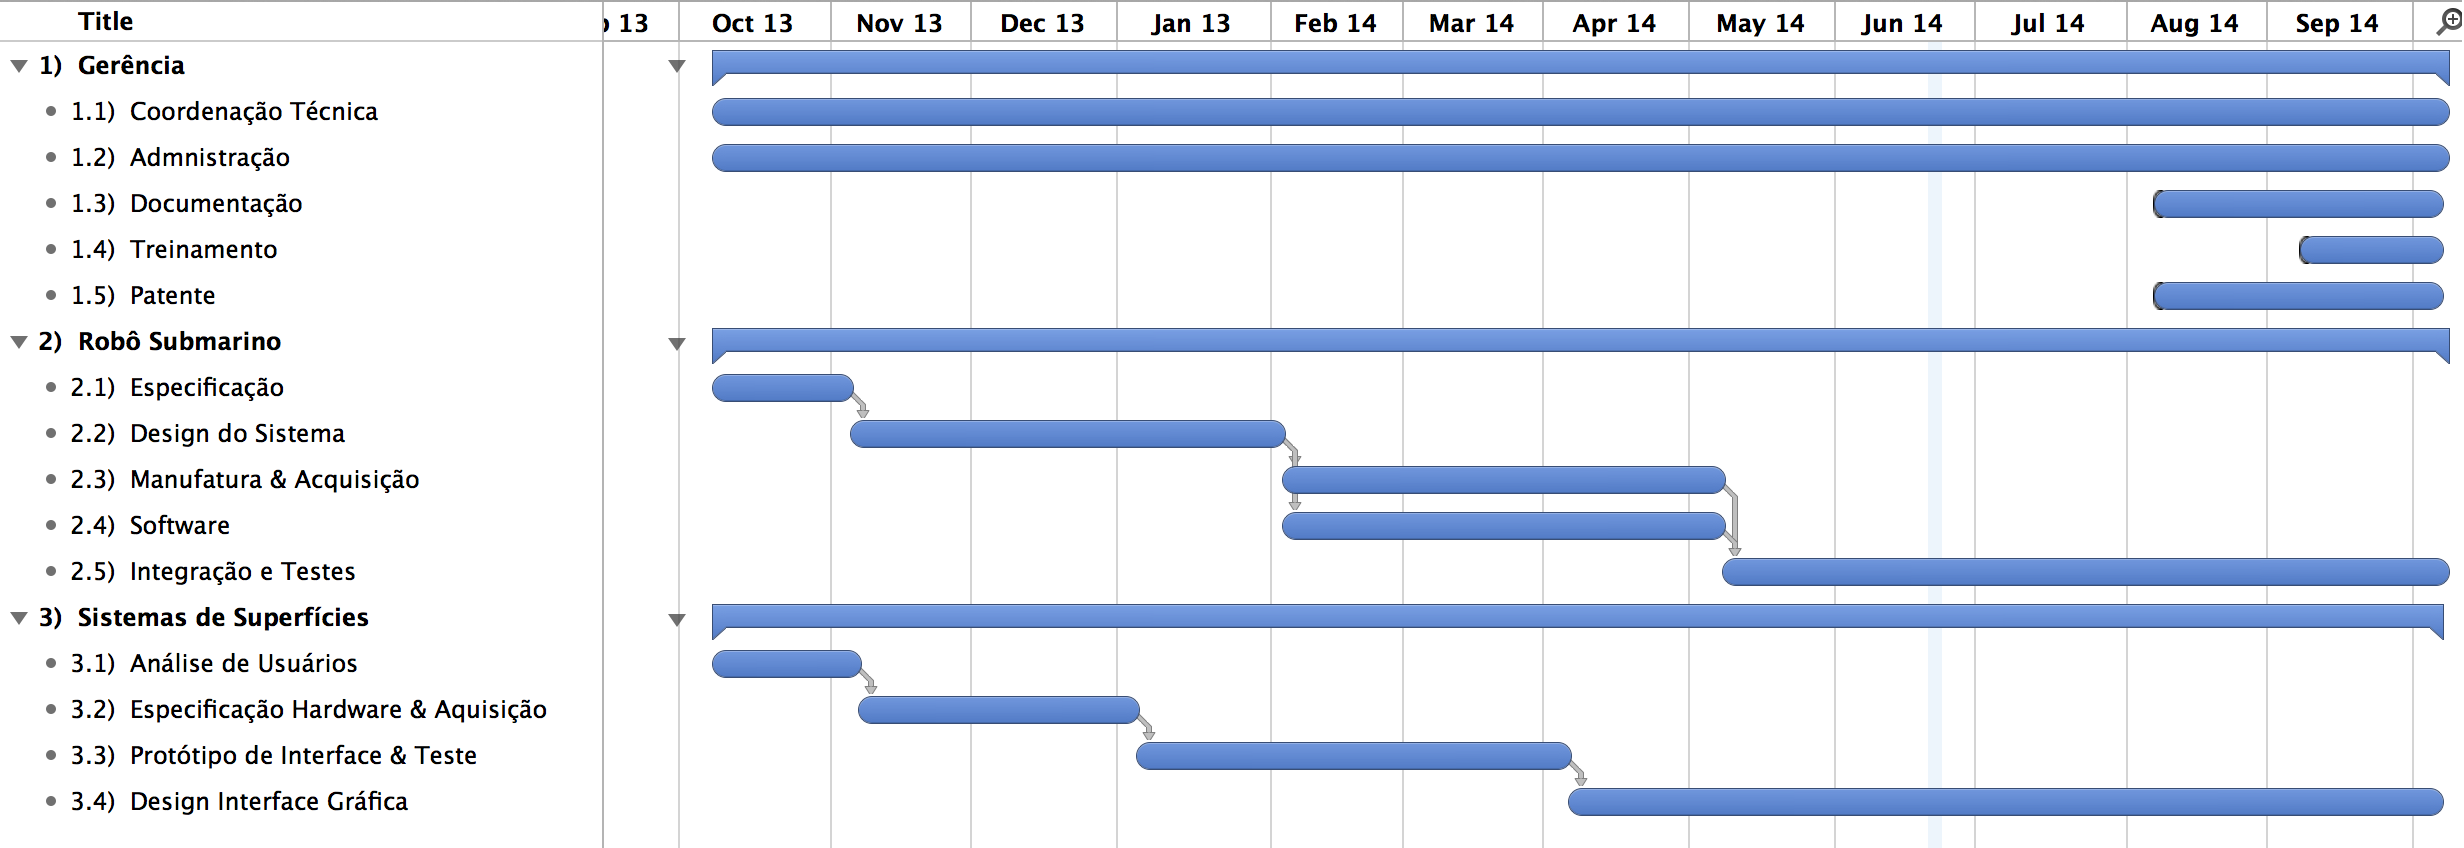
\includegraphics[angle=0,scale=0.40]{figs/gantt/Gantt_Original.png}
    \caption{Gantt Original.}
 
\end{figure}

\begin{figure}[h!]
 
  \centering

	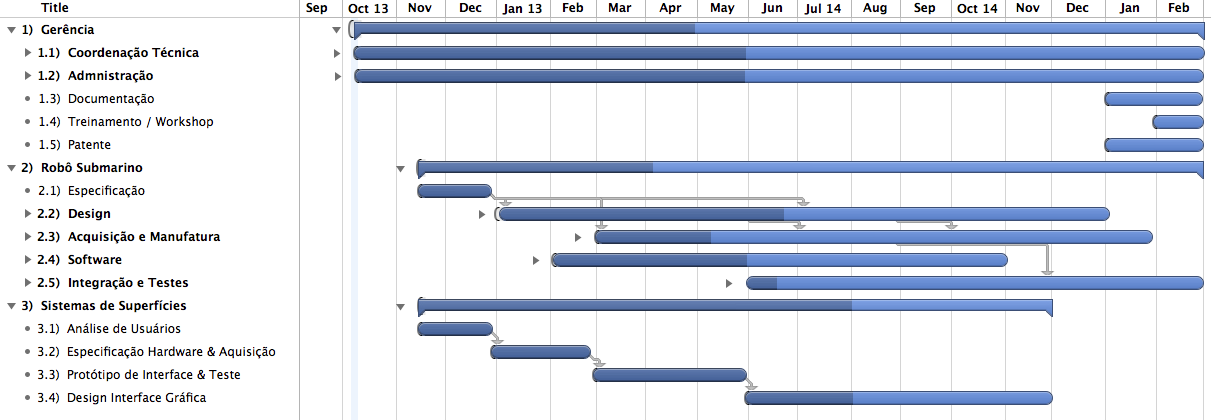
\includegraphics[angle=0,scale=0.40]{figs/gantt/Gantt_Atualisado.png}
    \caption{Gantt Atualisado.}
 
\end{figure}

\newpage 

\begin{figure}[h!]
 
  \centering

	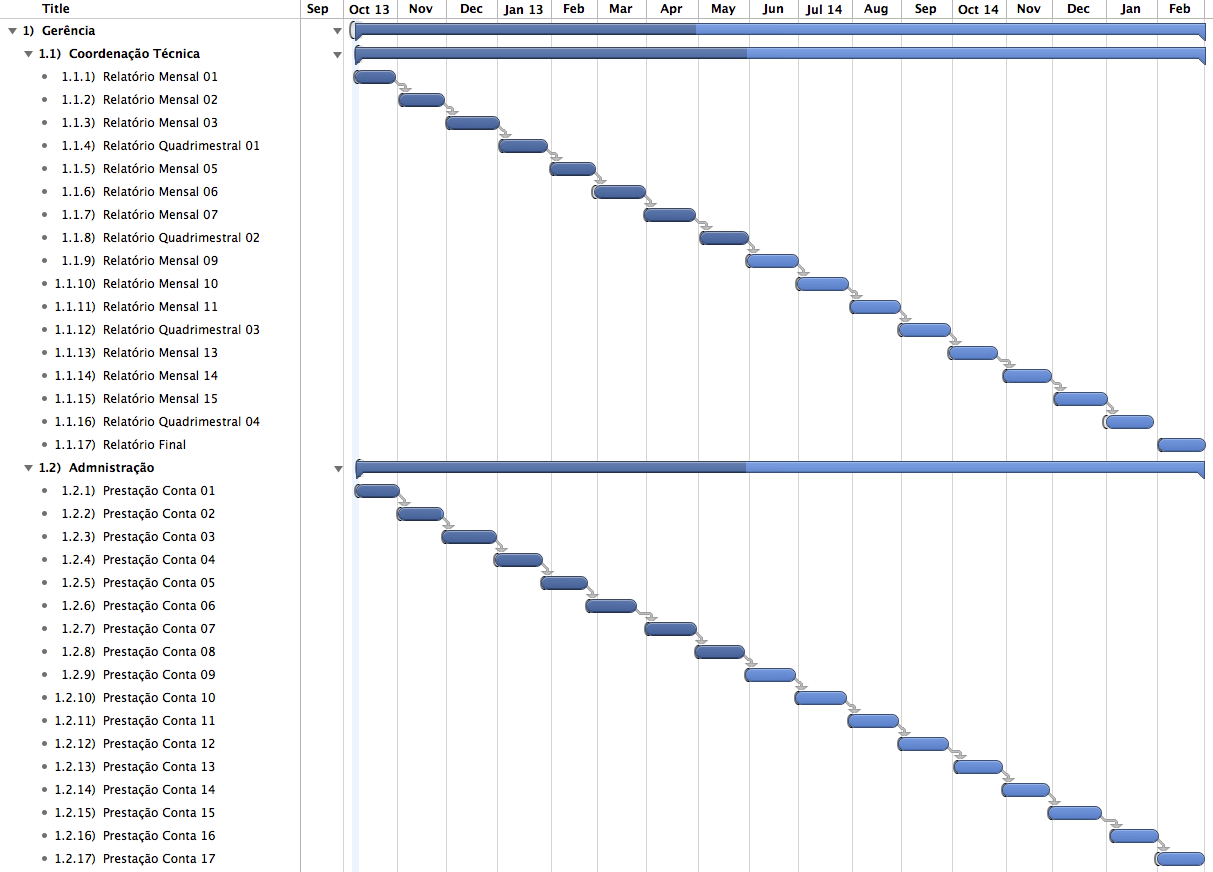
\includegraphics[angle=0,scale=0.40]{figs/gantt/Gantt_Detail_1.png}
    \caption{Gantt Detalhado Ger�ncia.}
 
\end{figure}

\newpage 

\begin{figure}[h!]
 
  \centering

	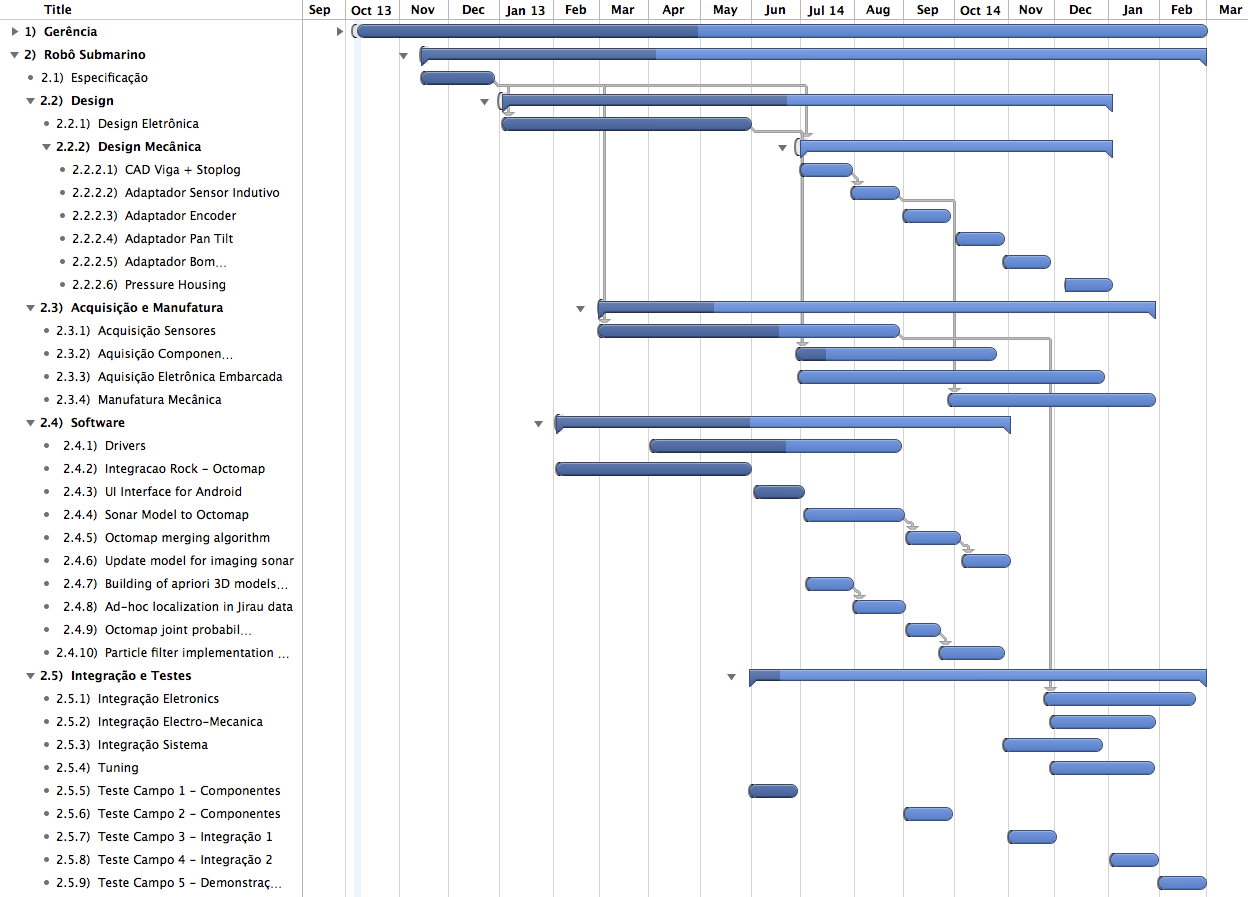
\includegraphics[angle=0,scale=0.40]{figs/gantt/Gantt_Detail_2.png}
    \caption{Gantt Detalhado Rob� Submarino.}
 
\end{figure}

\newpage

\subsection{Ger�ncia}

{\bf  1) Ger�ncia}: O planejamento tecnol�gico e administrativo, organiza��o, coordena��o e controle utilizados para alcan�ar os objetivos gerais do projeto, que n�o est�o associados a hardware espec�fico ou elementos de software.

\begin{description}

\item[1.1) Coordena��o T�cnica]: Coordenar a parte t�cnica do projeto, atribuindo tarefas e revendo o trabalho conclu�do.

\begin{description}
	\item [Original] - In�cio: Outubro 2013, Dura��o: 12 Meses 
	\item [Atualizado] - In�cio: Outubro 2014, Dura��o: 17 Meses
	\item [Raz�o] - A extens�o de 5 meses no plano de execu��o do projeto resulta na necessidade de se estender o tempo de dura��o da tarefa de coordena��o t�cnica pelo mesmo per�odo de tempo. 
\end{description}


\item[1.2) Administra��o]:  Administrar a parte financeira do projeto. 

\begin{description}
	\item [Original] - In�cio: Outubro 2013, Dura��o: 12 Meses 
	\item [Atualizado] - In�cio: Outubro 2014, Dura��o: 17 Meses
	\item [Raz�o] - A extens�o de 5 meses no plano de execu��o do projeto resulta na necessidade de se estender o tempo de dura��o da tarefa de administra��o pelo mesmo per�odo de tempo. 
\end{description}


	\item[1,3) Documenta��o:] Este pacote de trabalho lida com a escrita da documenta��o t�cnica e de opera��es. 

\begin{description}
	\item [Original] - In�cio: Agosto 2014, Dura��o: 2 Meses 
	\item [Atualizado] - In�cio: Janeiro 2014, Dura��o: 2 Meses
	\item [Raz�o] - O in�cio da tarefa precisa ser postergada, pois a execu��o deste pacote de trabalho � dependente da conclus�o da pesquisa do projeto que sofreu atrasos. 
\end{description}

	\item[1,4) Treinamento:] Esfor�o necess�rio para treinar o pessoal de opera��o da hidrel�tricas no uso do  sistema rob�tico desenvolvido no projeto.

\begin{description}
	\item [Original] - In�cio: Setembro 2014, Dura��o: 1 M�s 
	\item [Atualizado] - In�cio: Fevereiro 2014, Dura��o: 1 M�s
	\item [Raz�o] - O inicio da tarefa precisa ser postergada, pois a execu��o deste pacote de trabalho � dependente da conclus�o da pesquisa do projeto que sofreu atrasos. 
\end{description}

	\item[1,5) Patente:] Solicita��o de patente de produto para o sistema rob�tico desenvolvido.

\begin{description}
	\item [Original] - In�cio: Agosto 2014, Dura��o: 2 Meses 
	\item [Atualizado] - In�cio: Janeiro 2014, Dura��o: 2 Meses
	\item [Raz�o] - O in�cio da tarefa precisa ser postergada, pois a execu��o deste pacote de trabalho � dependente da conclus�o da pesquisa do projeto que sofreu atrasos. 
\end{description}

\end{description}

\subsection{Rob� Submarino}

\begin{description}

\vspace{0,5cm}

\item[ 2)  Rob� Submarino:] Este elemento lida com o trabalho necess�rio para desenvolver o sistema eletromec�nico do rob�.

\item[2,1) Especifica��o:] Neste pacote de trabalho, requisitos do sistema ser�o especificados atrav�s de reuni�es com os funcion�rios respons�veis pela opera��o na hidroel�trica e atrav�s de observa��es em campo. O resultado ser� um documento com os requisitos do sistema.

\begin{description}
	\item [Original] - In�cio: Outubro 2013, Dura��o: 1,5 Meses 
	\item [Atualizado] - In�cio: Novembro 2013, Dura��o: 1,5 Meses
	\item [Raz�o] - Devido a atrasos administrativos internos, a equipe do projeto s� foi contratada para trabalhar no projeto a partir do dia 18 de Novembro de 2013 o que resultou em um atraso equivalente para o in�cio da execu��o do pacote de trabalho 
\end{description}

\item[2,2) Design do Sistema:] Processo de defini��o da arquitetura, componentes, m�dulos e interface que satisfazem os requisitos do sistema.

\begin{description}
	\item [Original] - In�cio: Novembro 2013, Dura��o: 3 Meses 
	\item [Atualizado] - In�cio: Jan 2014, Dura��o: 12 Meses
	\item [Raz�o] - A tarefa design � dependente da tarefa Especifica��o (item 2.1), logo a mesma sofre uma posterga��o na data de in�cio. A tarefa design � composta por duas sub-tarefas: design eletr�nica e design mec�nica que eram para ser executadas em paralelo por um per�odo de 3 meses.

	\begin{description}

		 \item [Design Eletr�nica] O design da eletr�nica sofreu uma altera��o na dura��o para 6 meses. Pois, devido ao atraso no alinhamento admnistrativo, foi realizado 2 designs distintos da eletr�nica ao inv�s do �nico design inicialmente planejado. O design extra considerou a constru��o de uma eletr�nica com o equipamento emprestados de outros projetos do laborat�rio, o que permitiu a equipe de pesquisa seguir com as diversas tarefas dependentes da exist�ncia de uma eletr�nica, como o teste de campo realizado no in�cio de junho. 
	 
	  	\item [Design Mec�nico]
		 O design da mec�nica s� ser� iniciado em Julho de 2014 e a dura��o ser� de 6 meses. Pois, n�o foi poss�vel encontrar um engenheiro mec�nico com interesse e conhecimento em rob�tica para ser parte da equipe de pesquisa do projeto, logo foi necess�rio contratar o servi�o terceiro de Design Mec�nico. Entretanto, o processo de contrata��o s� se deu in�cio ap�s o problema de alinhamento administrativo do projeto ter sido resolvido, o que resultou no in�cio da sub-tarefa apenas em Julho 2014. A altera��o no prazo de dura��o da tarefa reflete a proposta da empresa contratada para a execu��o do servi�o.

	\end{description}

\end{description}


\item[2,3) Manufatura e Aquisi��o:] Compra e constru��o dos componentes definidos durante a fase de design do sistema. O resultado ser�o as partes que integradas formar�o o rob�.

\begin{description}
	\item [Original] - In�cio: Novembro 2013, Dura��o: 6 Meses 
	\item [Atualizado] - In�cio: Fevereiro 2014, Dura��o: 12 Meses
	\item [Raz�o] - O processo de aquisi��o de material permanente s� teve in�cio ap�s a resolu��o do problema de alinhamento administrativo entre a ESBR e a UFRJ, logo o pacote de trabalho s� teve in�cio em Fevereiro 2014. A dura��o do pacote de trabalho ser� de 12 meses ao inv�s de 3 meses, pois: 
	\begin{description}

		\item O sector de compras da funda��o COPPETEC entrou em processo de auditoria e permaneceu fechado por ?? Meses.  
		\item Erro na estimativa do tempo de entrega dos materiais planejados para o projeto, tempo m�ximo previsto de 3 meses, tempo estimado pelo fabricante 6 meses.  
		\item O processo de manufatura � dependente da tarefa design que sofreu atrasos (item 2.2). 

	\end{description}  
\end{description}

\item[2,4) Software:] Desenvolvimento de drivers, controladores e comunica��o para o hardware do rob�. O resultado ser� uma biblioteca de componentes do software.

\begin{description}
	\item [Original] - In�cio: Fevereiro 2014, Dura��o: 3 Meses 
	\item [Atualizado] - In�cio: Janeiro 2014, Dura��o: 10 Meses
	\item [Raz�o] - A tarefa teve seu in�cio adiantado e sofreu uma altera��o no prazo de dura��o, pois: 
     
     \begin{description}
		 \item O desenvolvimento dos drivers para os sensores e algoritmos de processamento do sonar s�o dependentes da entrega do equipamento, logo dependente da tarefa Aquisi��o (item 2.3) que se encontra atrasada.
		 \item A complexidade de se integrar o software de representa��o volum�trica (octomap) ao framework de rob�tica escolhido como plataforma foi subestimada na estimativa inicial do projeto. 
		 \item A complexidade da tarefa de processamento de dados sonar foi subestimada na estimativa inicial do projeto. 
	 \end{description} 

\end{description}

\item[2,5) - Integra��o e Teste:] Os componentes eletr�nicos, mec�nicos e de software ser�o integrado no sistema Viga Pescadora Inteligente. Este pacote de trabalho tamb�m inclui a instala��o e teste do sistema.

\begin{description}
	\item [Original] - In�cio: Maio 2014, Dura��o: 5 Meses 
	\item [Atualizado] - In�cio: Junho 2014, Dura��o: 9 Meses
	\item [Raz�o] - A tarefa � dependente das tarefas Aquisi��o e Manufatura (item 2.3) e Software (2.4) que se encontram atrasadas, logo a mesma sofreu atrasos equivalentes em sua execu��o. 

\end{description}

\end{description}


\subsection{Sistemas de Superf�cie}

\begin{description}

\item[3) Sistemas de Superf�cie:] Este elemento inclui o hardware e o software necess�rios para a opera��o do rob� na superf�cie, incluindo a concep��o, desenvolvimento, implementa��o e integra��o da comunica��o, interface e ger�ncia de dados.

\item[3,1) An�lise de Usu�rio:] An�lise dos potenciais usu�rio do sistemas. Este pacote de trabalho vai resultar em um documento que define: O que o usu�rio espera do sistema. Como o sistema ir� fazer parte do dia a dia da opera��o. Qual � a capacita��o t�cnica do futuro usu�rio. Qual apar�ncia de interface t�m um maior apelo para o usu�rio.

\begin{description}
	\item [Original] - In�cio: Outubro 2013, Dura��o: 1,5 Meses 
	\item [Atualizado] - In�cio: Novembro 2013, Dura��o: 1,5 Meses
	\item [Raz�o] - Devido a atrasos administrativos internos, a equipe do projeto s� foi contratada para trabalhar no projeto a partir do dia 18 de Novembro de 2013 o que resultou em um atraso equivalente para o in�cio da execu��o do pacote de trabalho

\end{description}

\item[3,2) Especifica��o de Hardware e Aquisi��o:] Este pacote de trabalho inclui a especifica��o e aquisi��o do equipamento necess�rio para operar o rob� a partir da superf�cie. O resultado � um lista de componentes, e respectivos fabricantes, a serem comprados para o projeto.


\begin{description}
	\item [Original] - In�cio: Novembro 2013, Dura��o: 2 Meses 
	\item [Atualizado] - In�cio: Janeiro 2014, Dura��o: 2 Meses
	\item [Raz�o] - A tarefa precisa ser postergada, pois a execu��o deste pacote de trabalho � dependente da conclus�o da tarefas An�lise de Usu�rio (item 3.1) que sofreu atrasos. 

\end{description}


\item[3,3) Prot�tipo de Interface e Teste:] Desenvolvimento de telas interativas simples, sem conte�do, concentrando apenas no desenvolvimento da parte visual da interface. Estes prot�tipo de interface vai ser testado com os futuros usu�rio dos sistema e o resultado da sensa��o da mesma ser� avaliada.

\begin{description}
	\item [Original] - In�cio: Janeiro 2014, Dura��o: 3 Meses 
	\item [Atualizado] - In�cio: Marco 2013, Dura��o: 3 Meses
	\item [Raz�o] - A tarefa precisa ser postergada, pois a execu��o deste pacote de trabalho � dependente da conclus�o da tarefas Especifica��o de Hardware e Aquisi��o (item 3.2) que sofreu atrasos. 

\end{description}

\item[3,4) Interface de Usu�rio:] Implementa��o da interface de usu�rio (GUI) do rob�, o que permite a visualiza��o e o seu controle. O resultado ser� um software.

\begin{description}
	\item [Original] - In�cio: Abril 2014, Dura��o: 6 Meses 
	\item [Atualizado] - In�cio: Junho 2014, Dura��o: 6 Meses
	\item [Raz�o] - A tarefa precisa ser postergada, pois a execu��o deste pacote de trabalho � dependente da conclus�o da tarefas Prot�tipo de Interface e Teste (item 3.3) que teve seu in�cio postergado. 

\end{description}

\end{description}


%%******************************************************************************
%% SECTION - Financeiro
%%******************************************************************************
\section{Financeiro}
\label{financeiro}

O relat�rio financeiro aqui apresentado t�m como objetivo demonstrar o que foi estimado no in�cio do projeto, o que foi at� o momento executado e a previs�o atual do desenbolso necess�rio at� o fim do projeto, fornecendo uma vis�o global do plano financeiro do projeto. Logo, as informa��es contidas neste  relat�rio ser�o diferentes das informa��es contidas no relat�rio financeiro de presta��o de contas, o qual detalha apenas os lan�amentos realizados na conta do projeto at� a data de fechamento do m�s. Por favor, notar que existem itens detalhados como executados neste relat�rio que n�o estar�o presentes na presta��o de contas. Isto ocorre devido a defasagem de tempo entre a decis�o de comprar o item e a data de pagamento da nota fiscal. Por mais, todos as informa��es presentes em ambos os relat�rios dever�o ser consistentes e em caso de inconsist�ncia o valor relatado no relat�rio de presta��o de contas dever ser considerado como o correto.

\subsection{Desembolso}

\begin{center}
  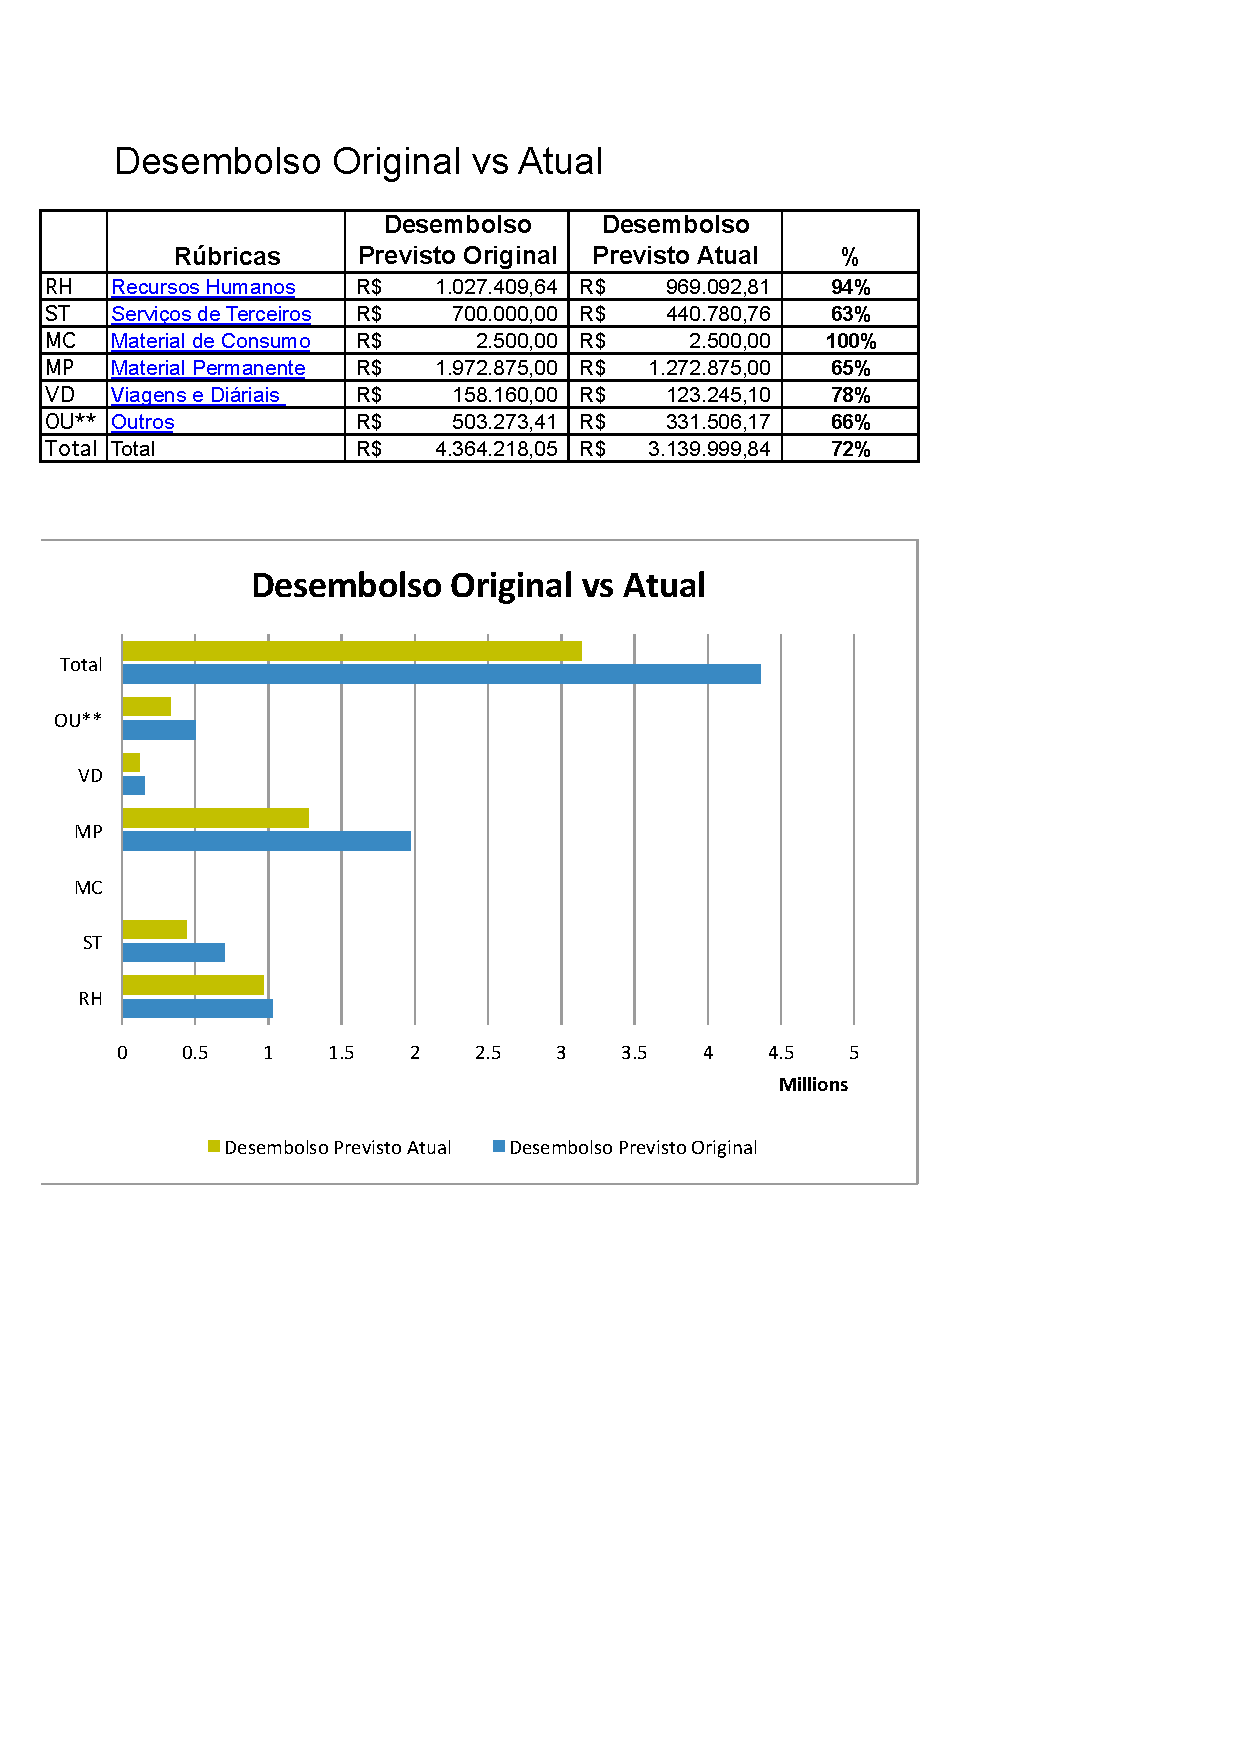
\includegraphics[width=\textwidth]{figs/financeiro/ROSA_Cronograma_Fisico_Financeiro_05_26_2014_Desenbolso.pdf}
\end{center}

\subsection{Recursos humanos}

\begin{center}
  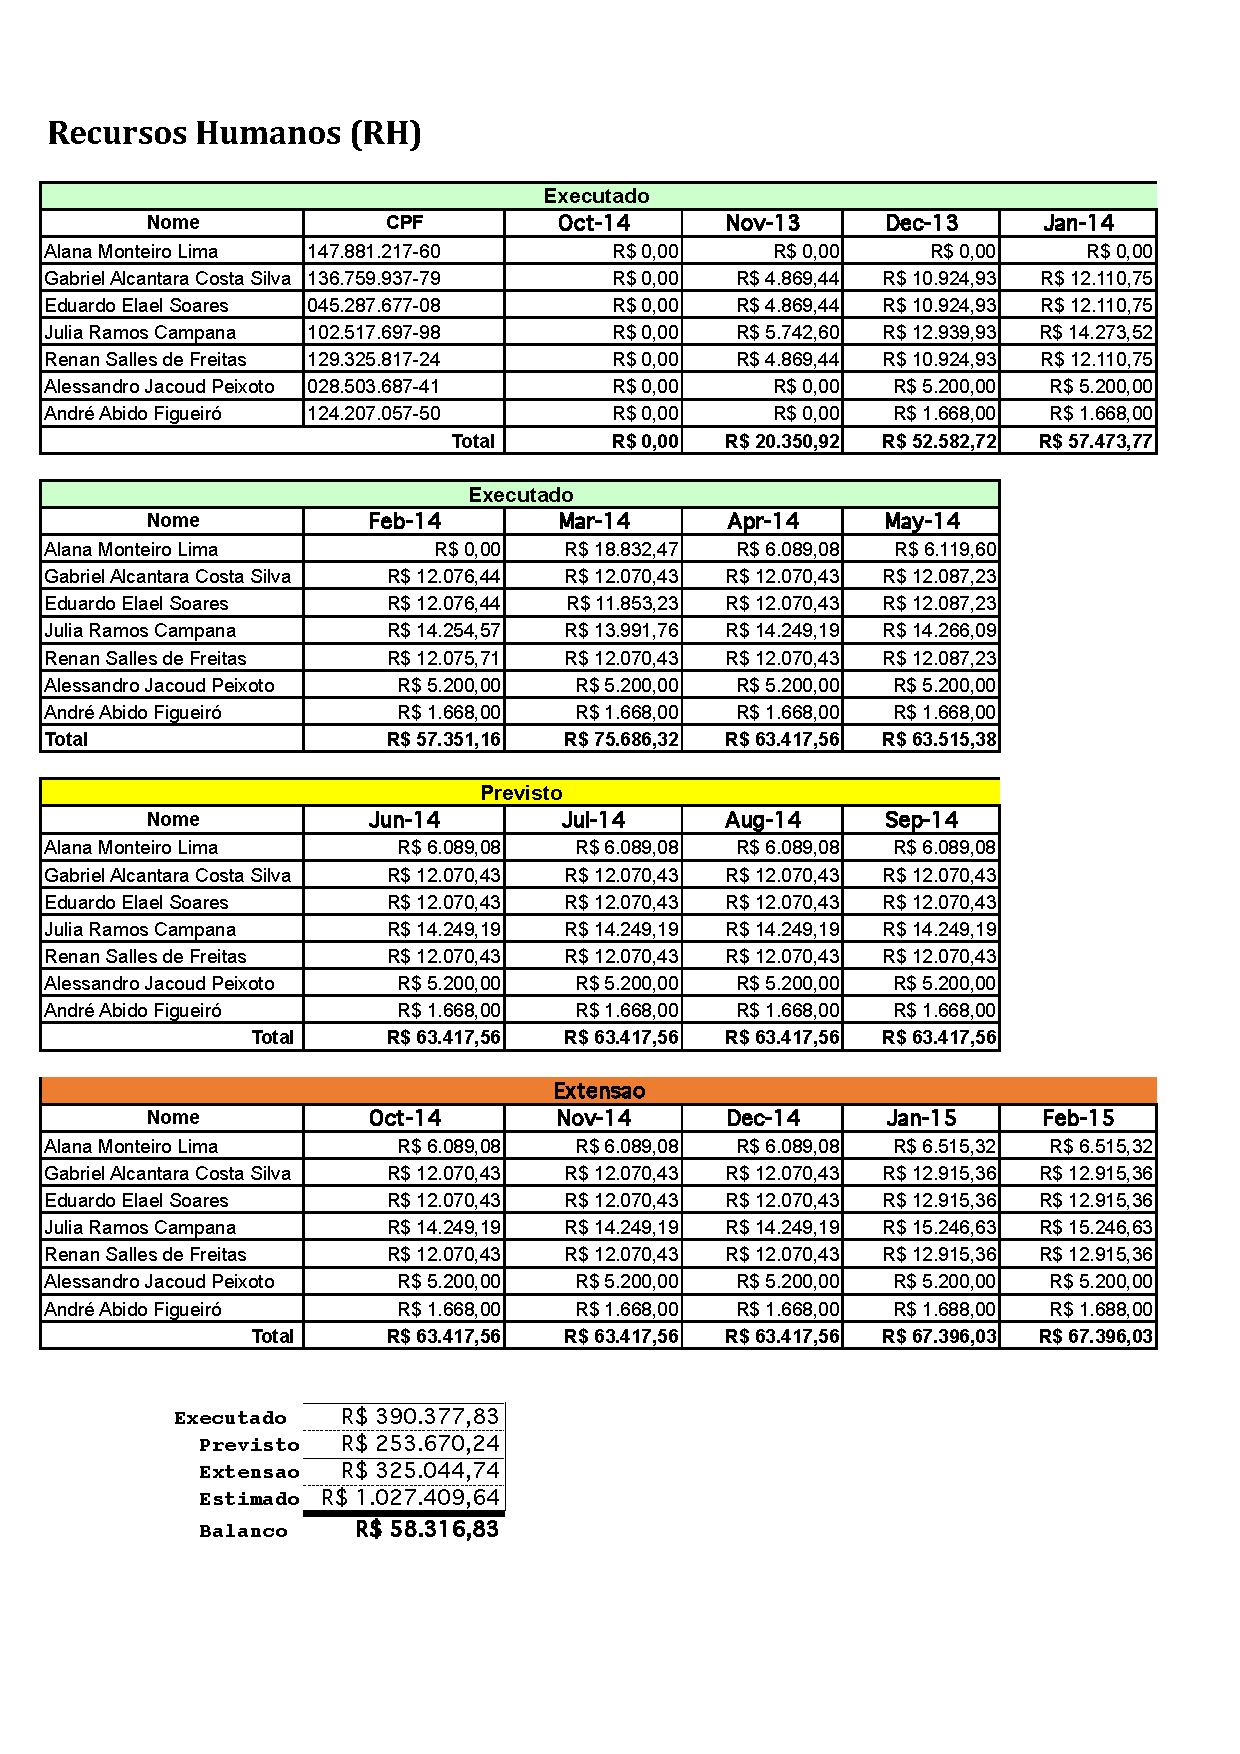
\includegraphics[width=1\columnwidth]{figs/financeiro/ROSA_Cronograma_Fisico_Financeiro_05_26_2014_RH.pdf}
\end{center}

\subsection{Servi�os de terceiros}

\begin{center}
  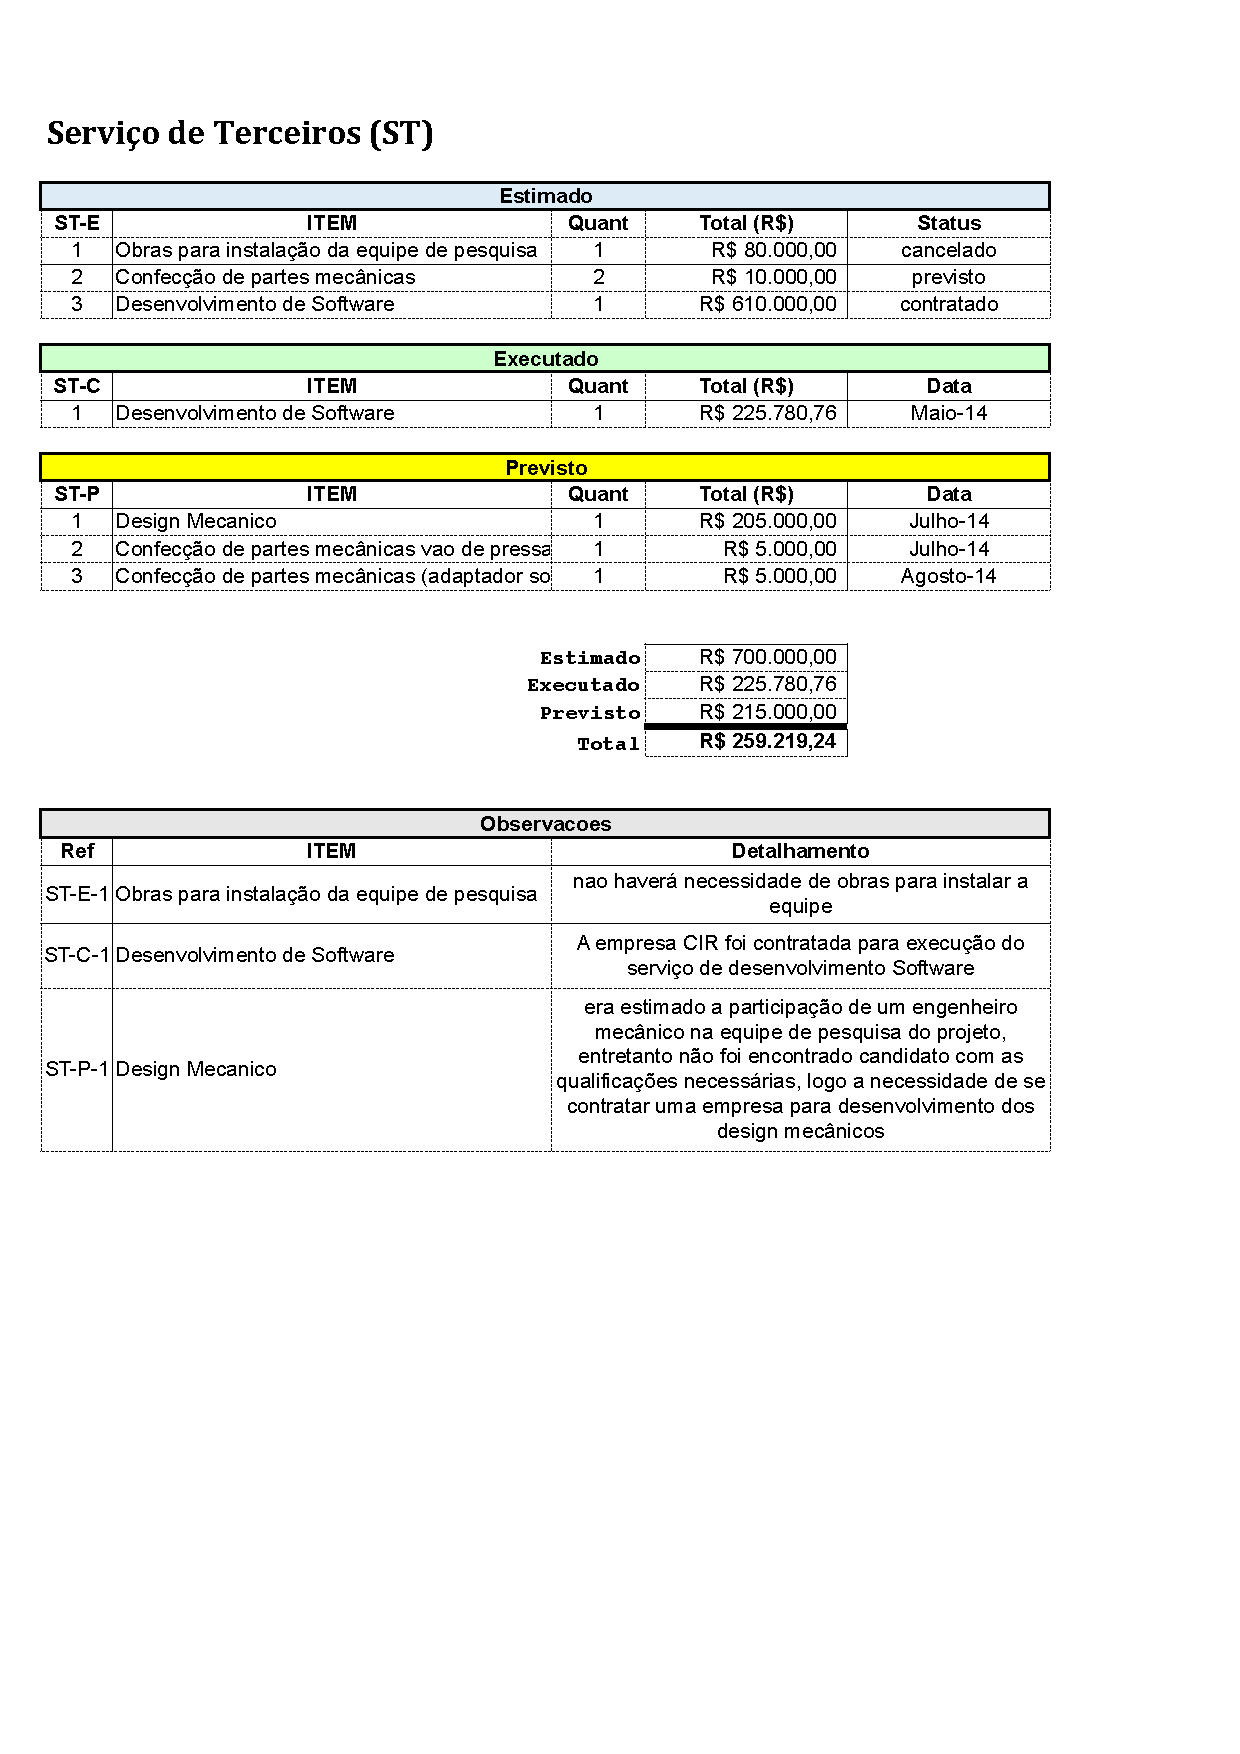
\includegraphics[width=1\columnwidth]{figs/financeiro/ROSA_Cronograma_Fisico_Financeiro_05_26_2014_ST.pdf}
\end{center}

\subsection{Material de consumo}

\begin{center}
  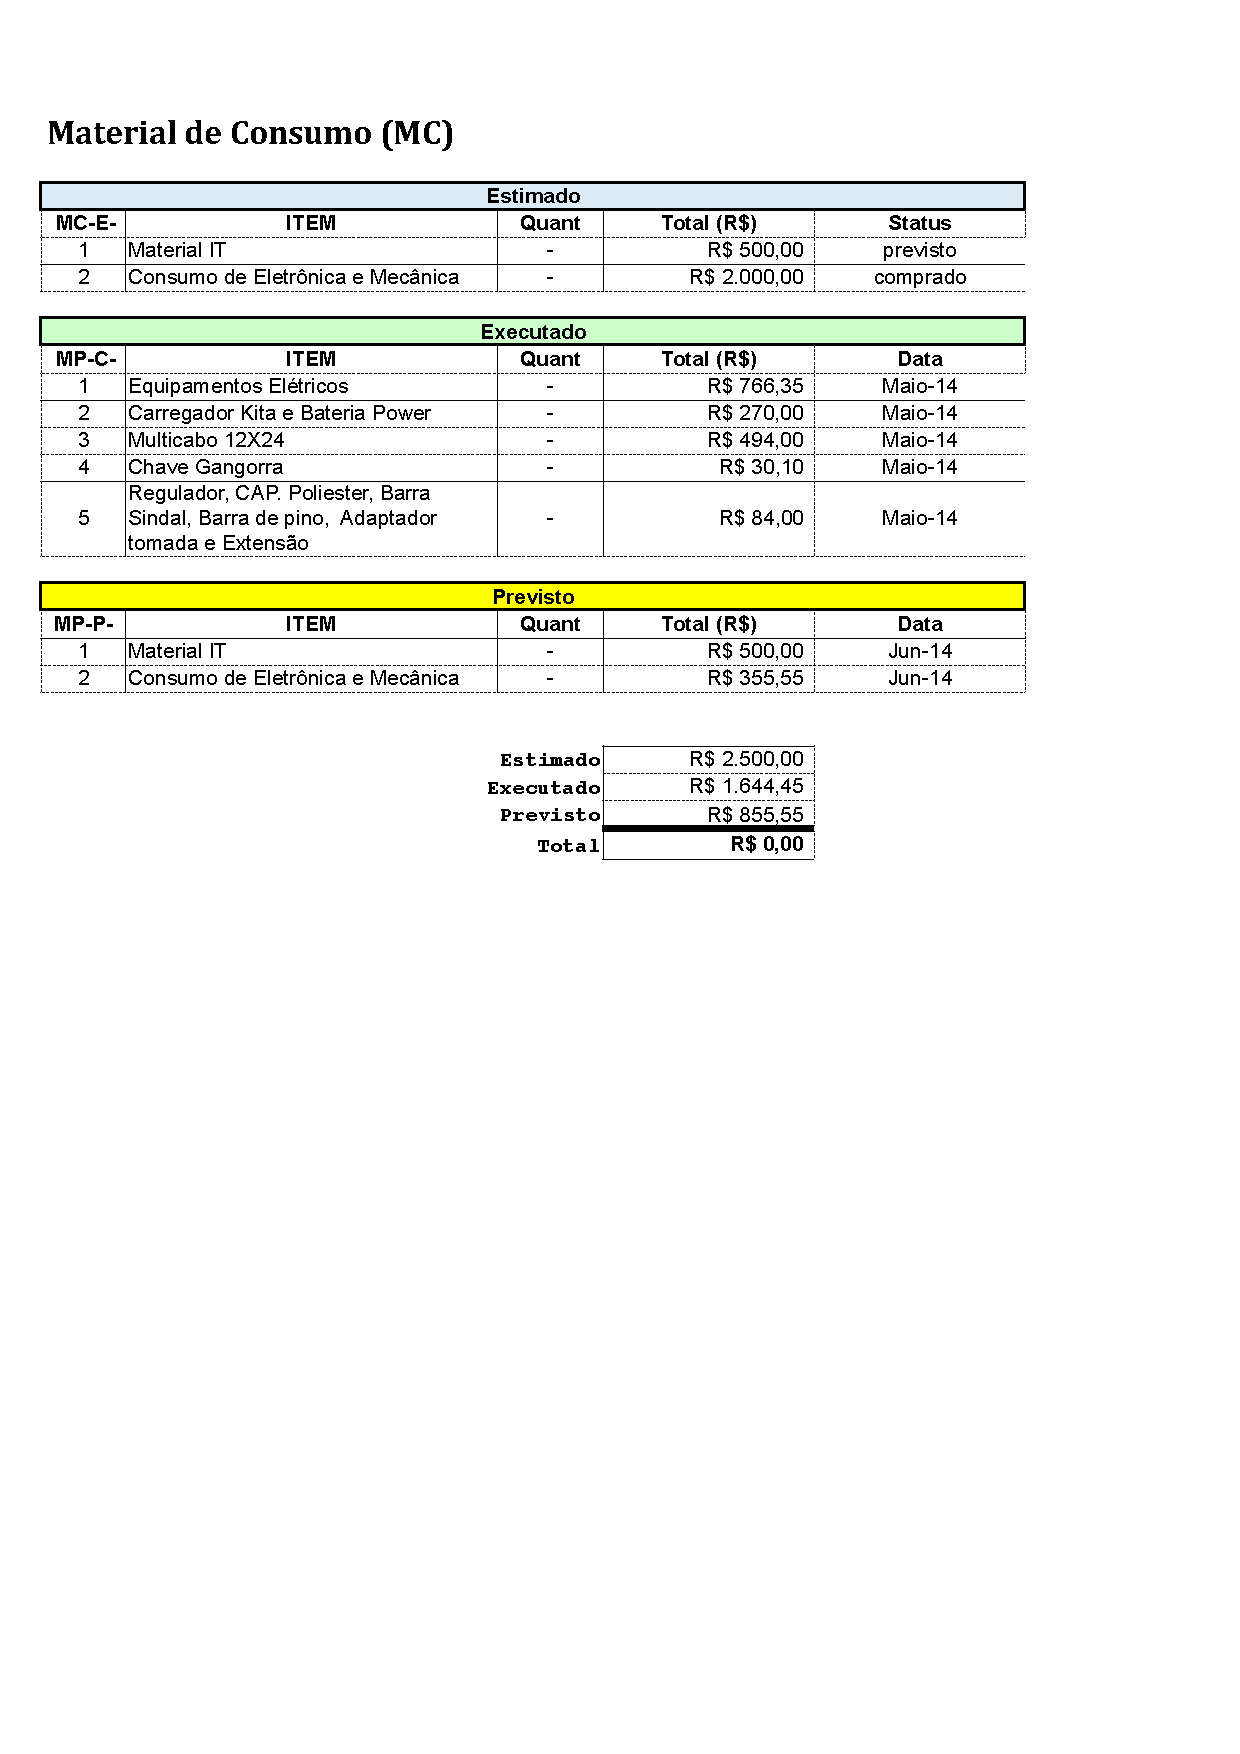
\includegraphics[width=1\columnwidth]{figs/financeiro/ROSA_Cronograma_Fisico_Financeiro_05_26_2014_MC.pdf}
\end{center}

\subsection{Material permanente}

\begin{center}
  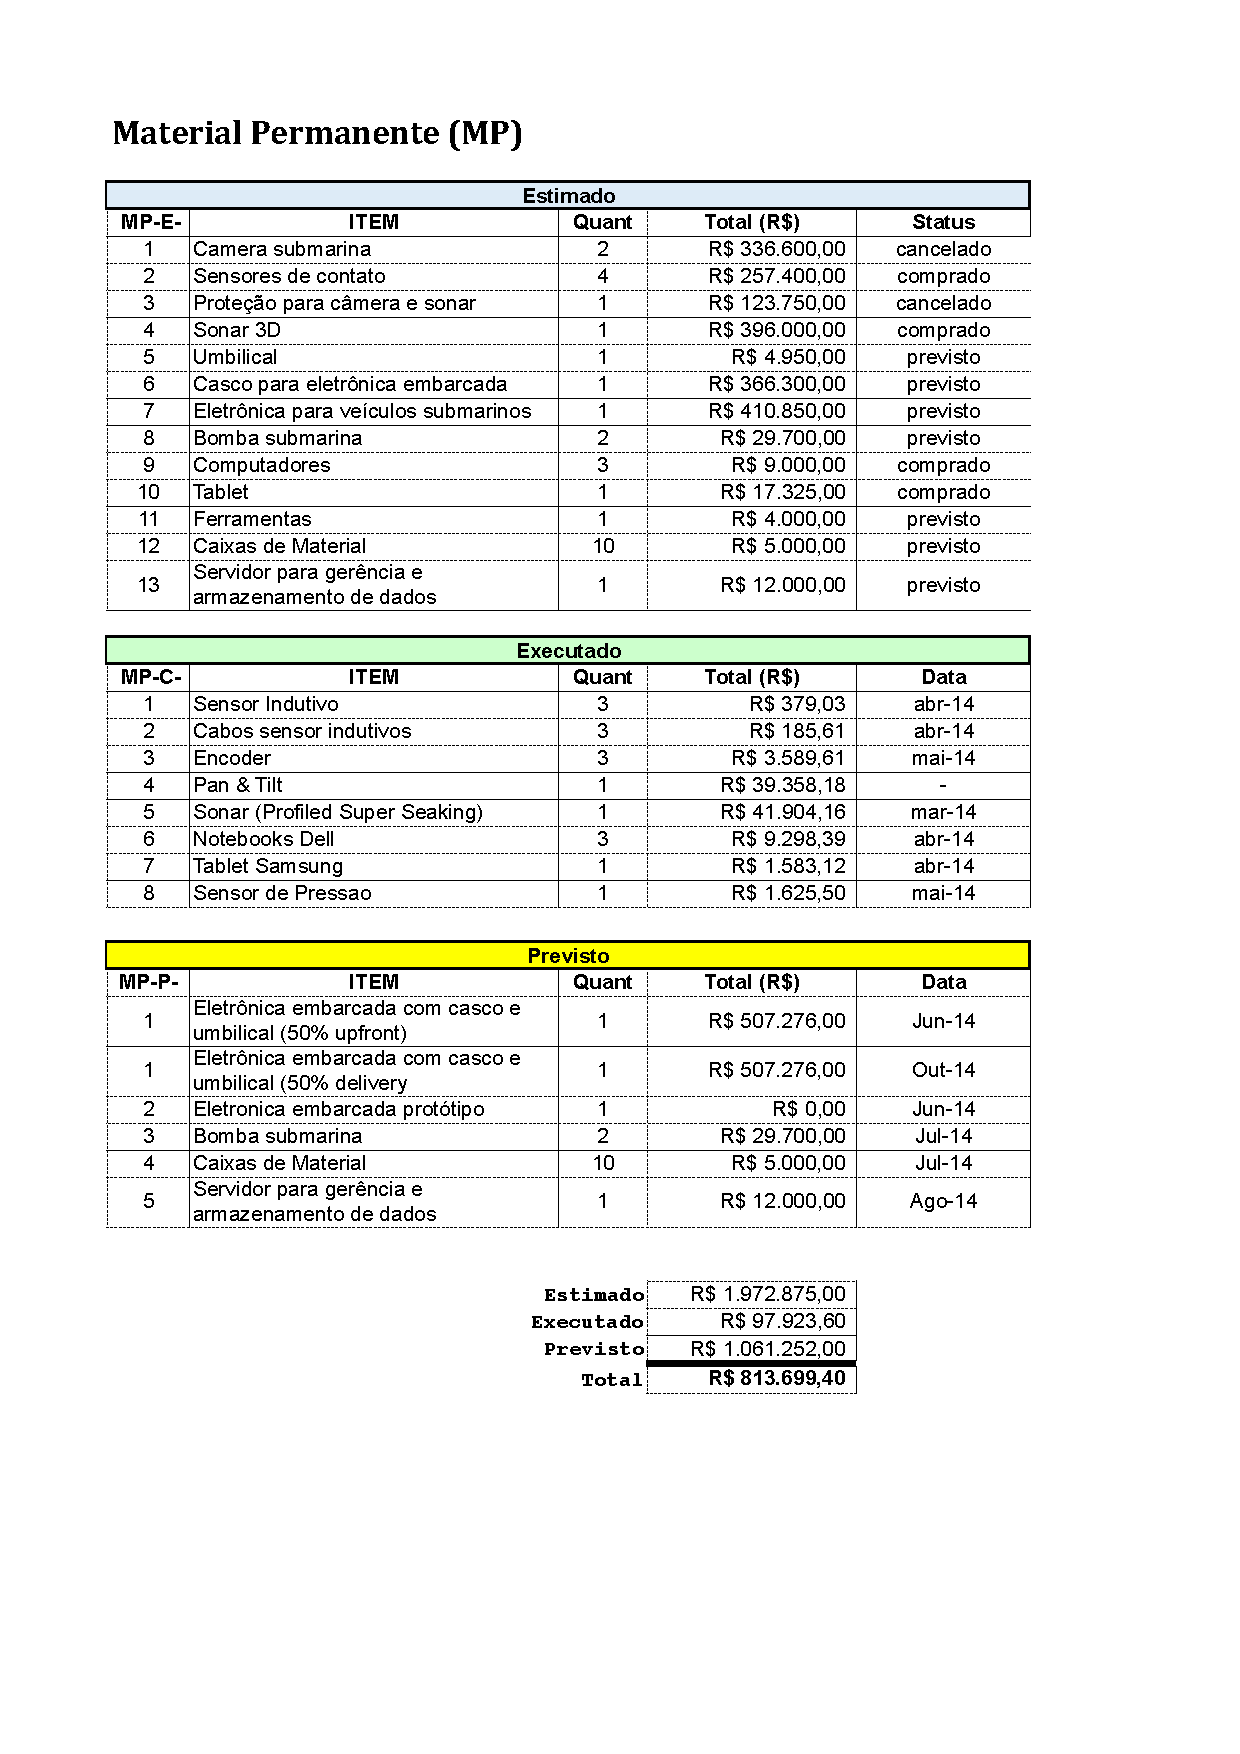
\includegraphics[width=1\columnwidth]{figs/financeiro/ROSA_Cronograma_Fisico_Financeiro_05_26_2014_MP.pdf}
\end{center}

\subsection{Viagens e di�rias}

\begin{center}
  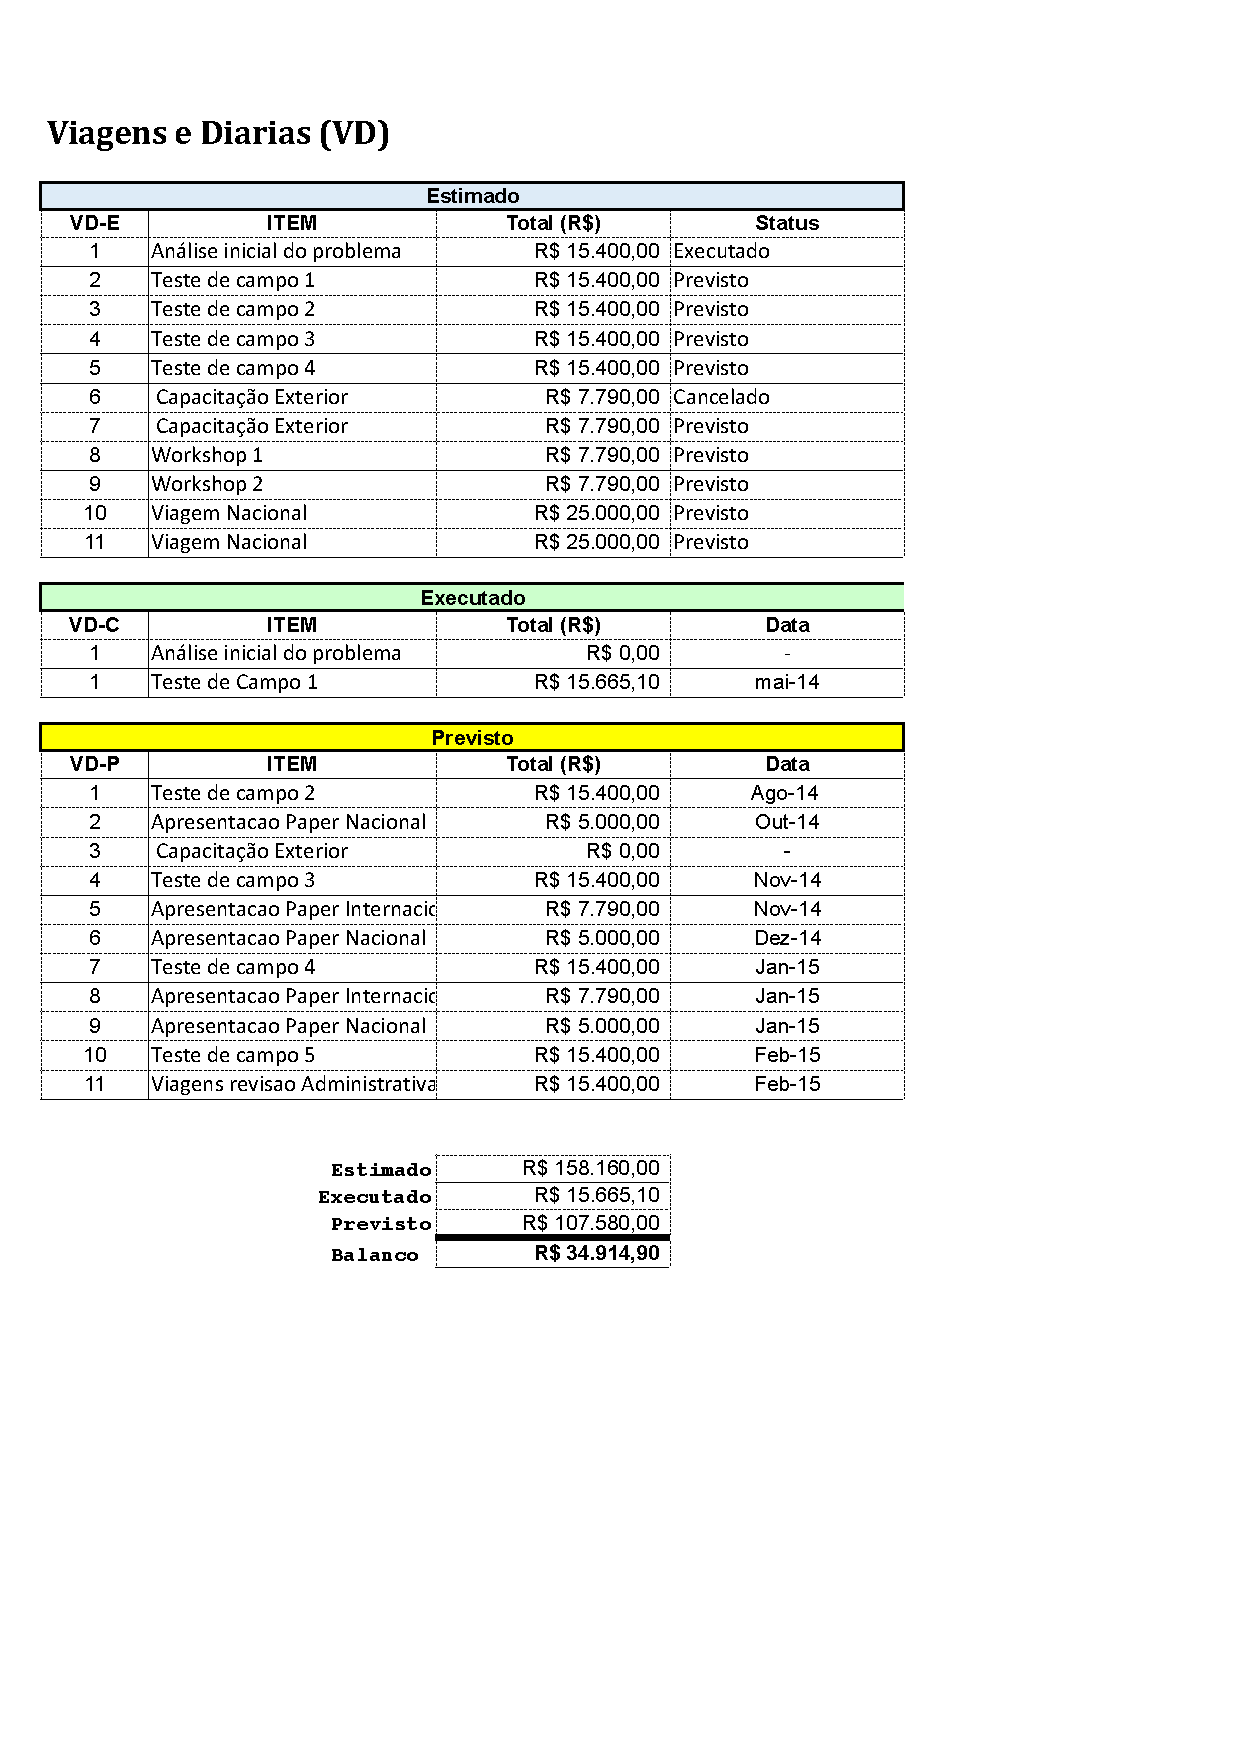
\includegraphics[width=1\columnwidth]{figs/financeiro/ROSA_Cronograma_Fisico_Financeiro_05_26_2014_VD.pdf}
\end{center}

\subsection{Outros}

\begin{center}
  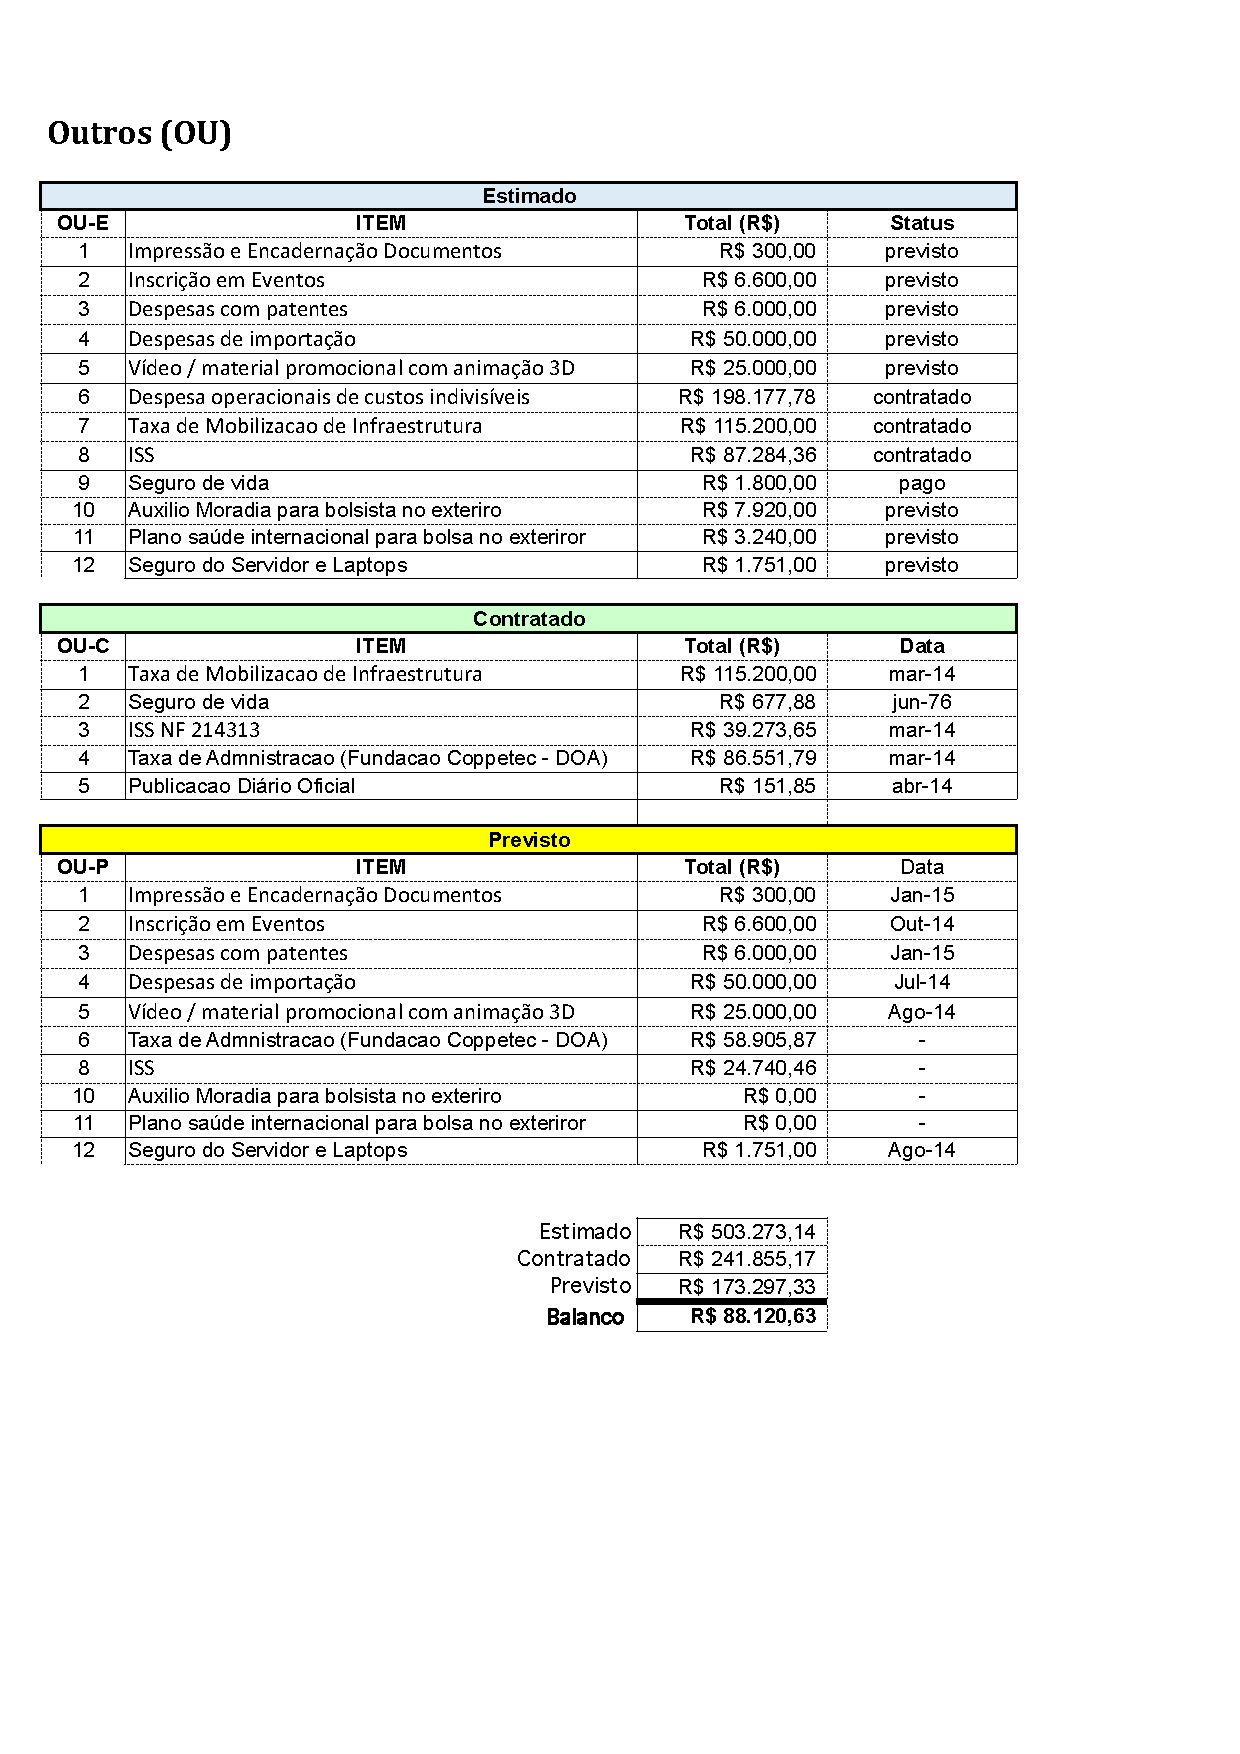
\includegraphics[width=1\columnwidth]{figs/financeiro/ROSA_Cronograma_Fisico_Financeiro_05_26_2014_Ou.pdf}
\end{center}

\subsection{Balan�o}

\begin{center}
  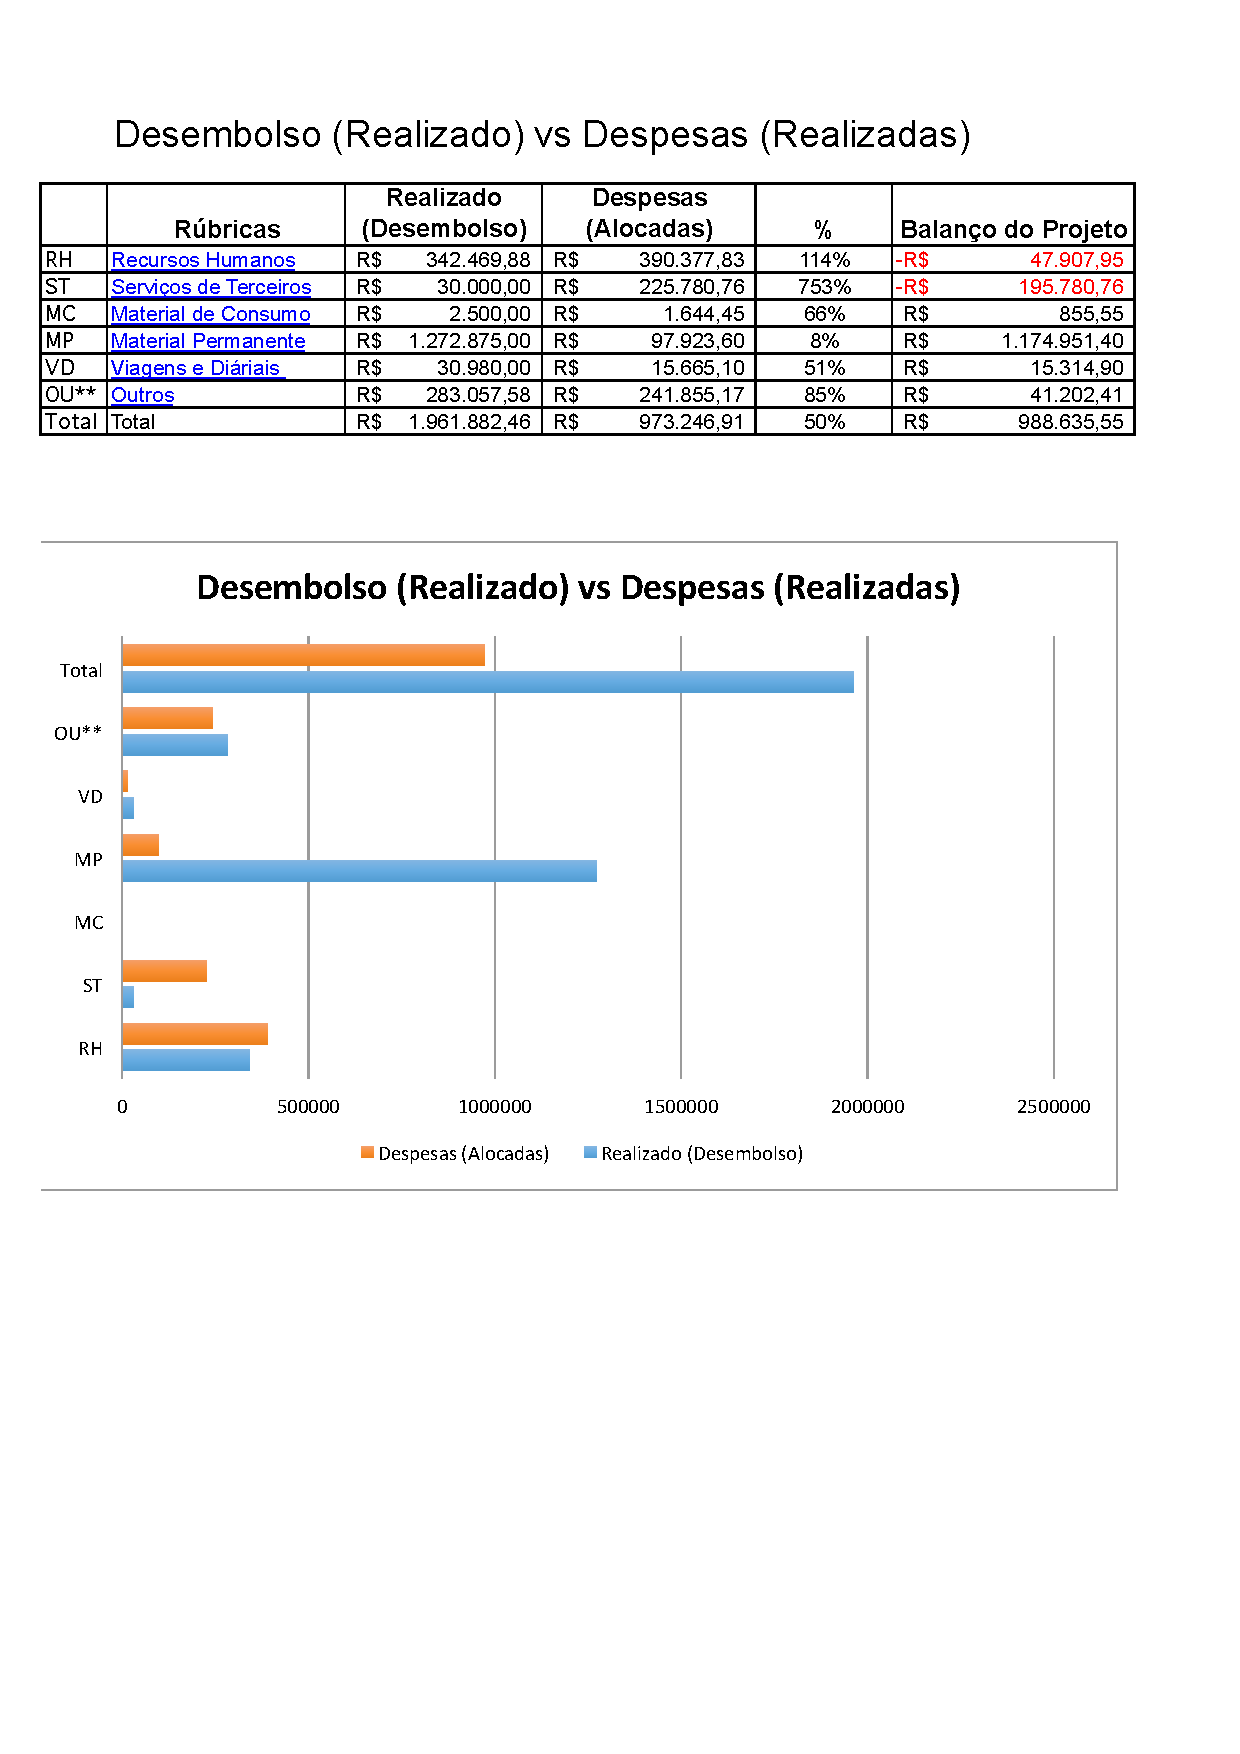
\includegraphics[width=1\columnwidth]{figs/financeiro/ROSA_Cronograma_Fisico_Financeiro_05_26_2014_Balanco.pdf}
\end{center}


\subsection{Cronograma}

\begin{center}
  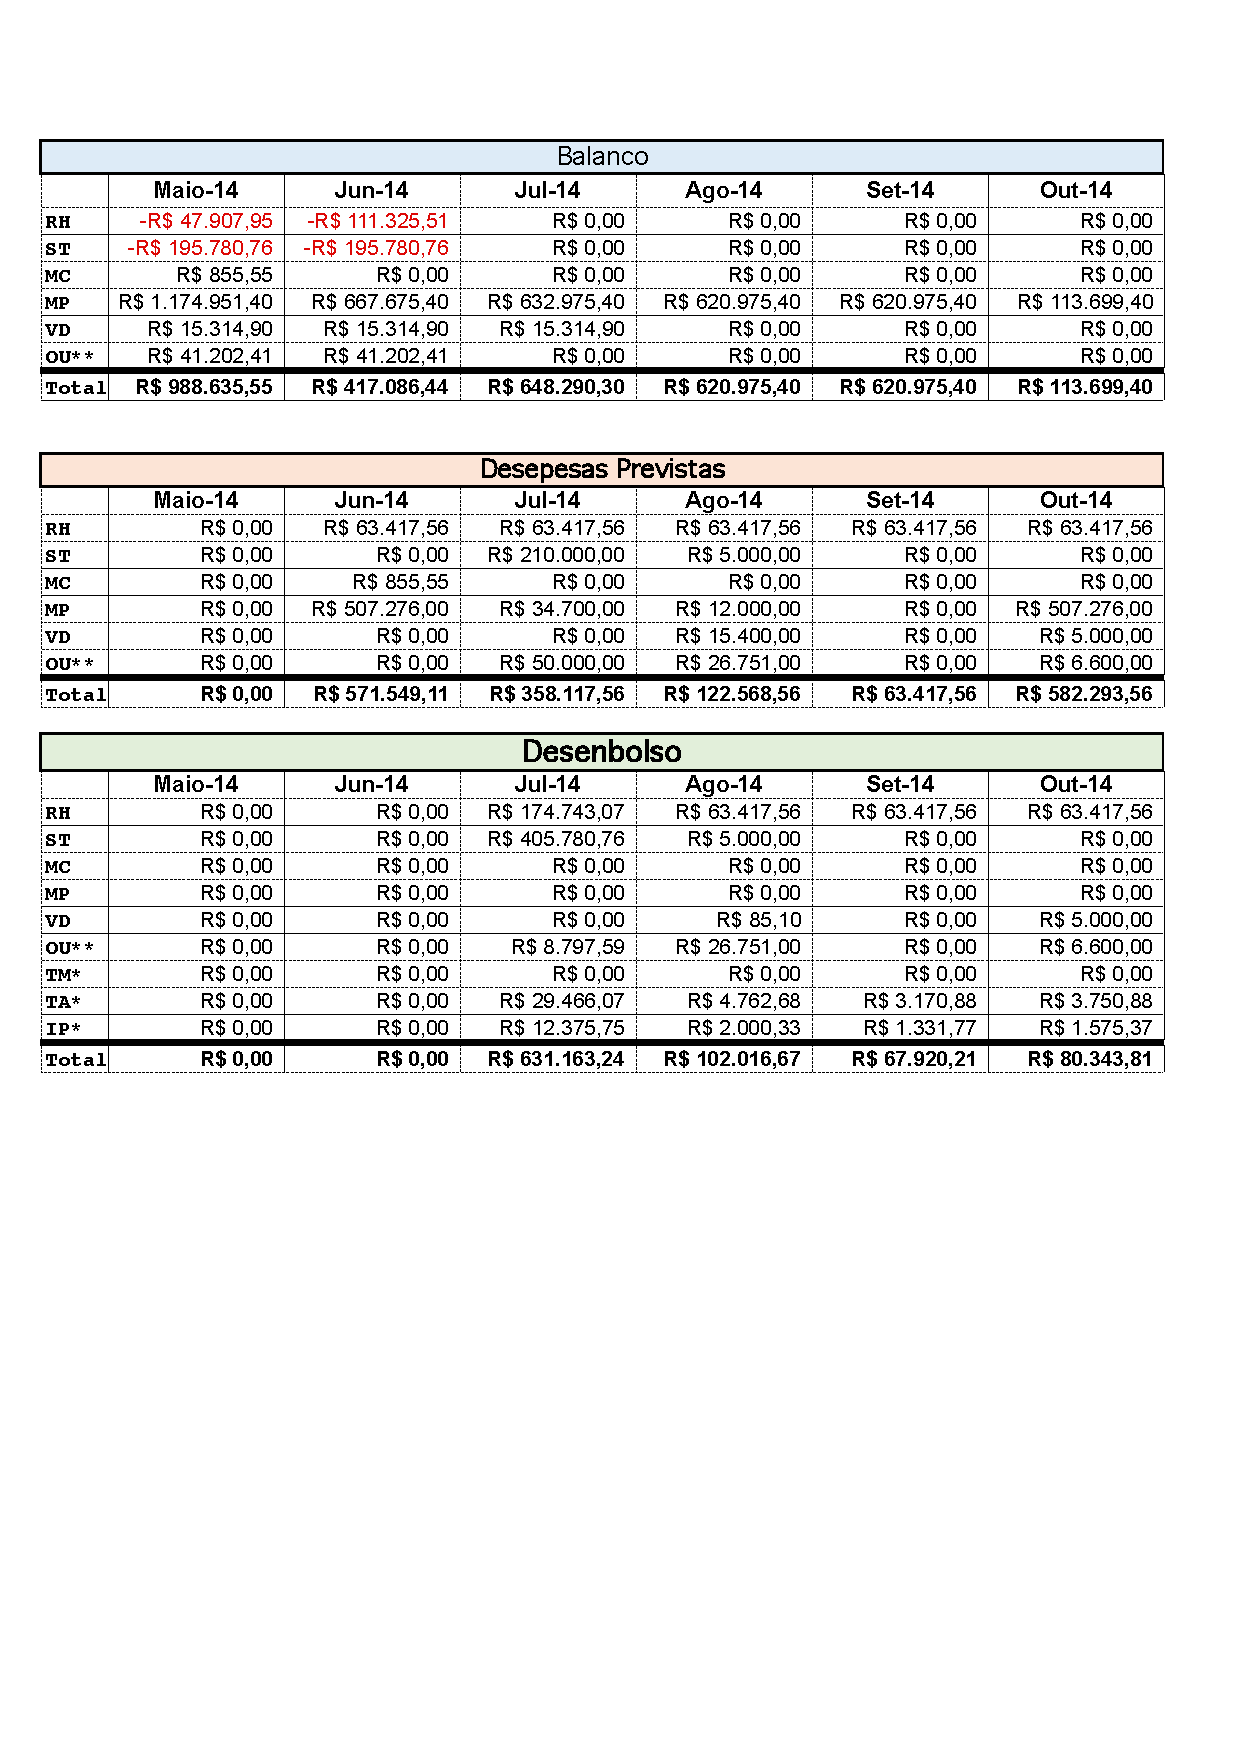
\includegraphics[width=1\columnwidth]{figs/financeiro/ROSA_Cronograma_Fisico_Financeiro_05_26_2014_Cronograma_Desenbolso.pdf}
\end{center}

\begin{center}
  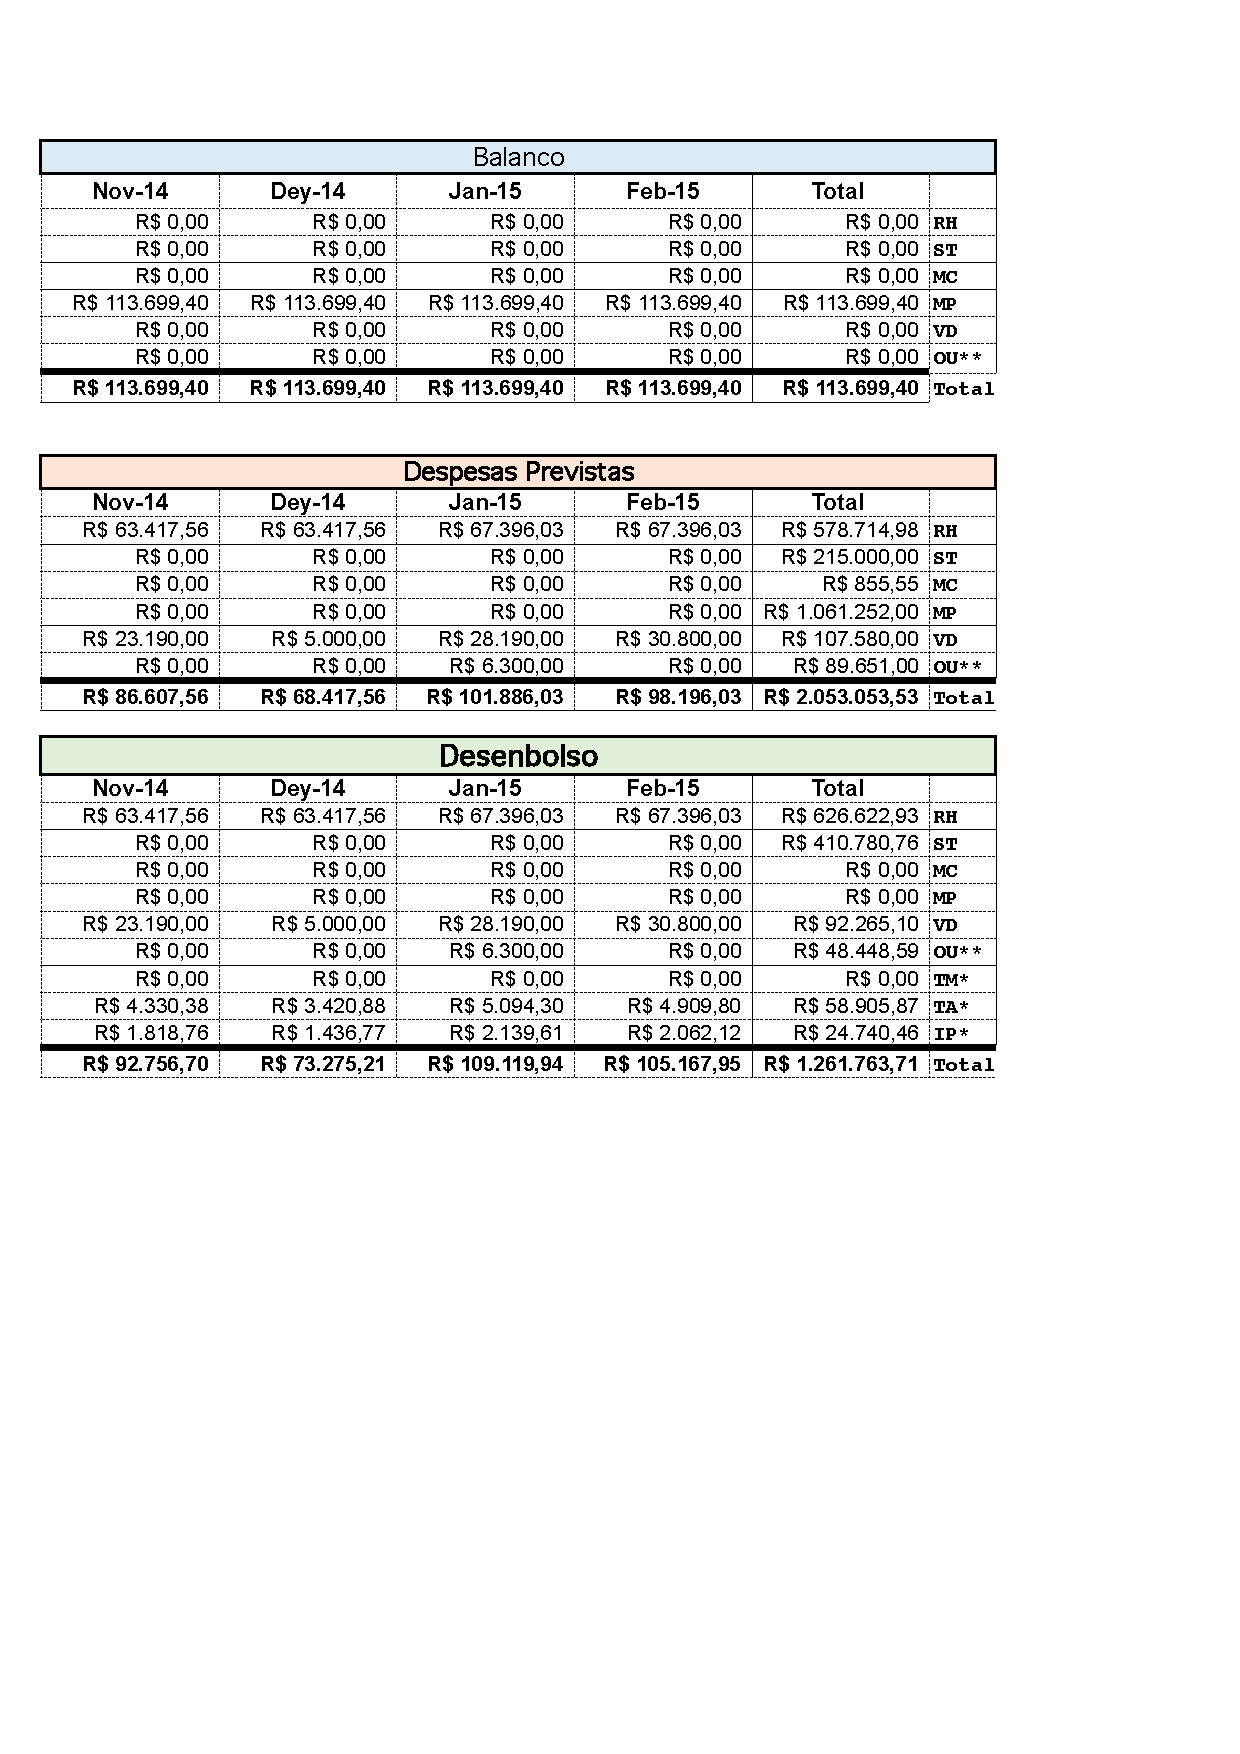
\includegraphics[width=1\columnwidth]{figs/financeiro/ROSA_Cronograma_Fisico_Financeiro_05_26_2014_Cronograma_Desenbolso_2.pdf}
\end{center}










%\newpage%
%---------------------------------------------------------------------
%%% \section{Minutas}
%%%
%%% \input{../minutas/minuta-de-reuniao(25-out-2013)} \newpage%
%%% \input{../minutas/minuta-de-reuniao(01-nov-2013)} \newpage%

%---------------------------------------------------------------------
\fim

%---------------------------------------------------------------------
\end{document}
